\section{Reconstruction of deposited energy and time in the MTD}
%editors: P. Meridiani & A. Benaglia
\label{C5Sec:mtdreco}
%\subsubsection{Energy and time reconstruction}
The energy deposited by a particle is reconstructed by clustering the energy deposits in adjacent cells matched to a track.  
A basic algorithm consists in summing the energy deposits -- above the readout threshold -- that lie within a cone of $\Delta R = 0.05$ around the extrapolation of track to the MTD surface. 
%[Note: this description is valid for the current plots. Text and the plots need to be updated to reflect the usage of clusters]. 
The distributions of the total energy deposit predicted for single muons and pions, and for minimum bias events are shown in Fig.~\ref{fig:BTL_Edep}-left for BTL and Fig.~\ref{fig:BTL_Edep}-right for ETL. 
Muons behave as MIP in the timing layer, and the most probable value of a Landau interpolation of the energy deposit distribution correspond to about 5~MeV in BTL and 0.15~MeV in ETL. In the case of hadrons, the distribution features a high energy tail ascribed to nuclear interactions.

\begin{figure}[hbtp]
\centering
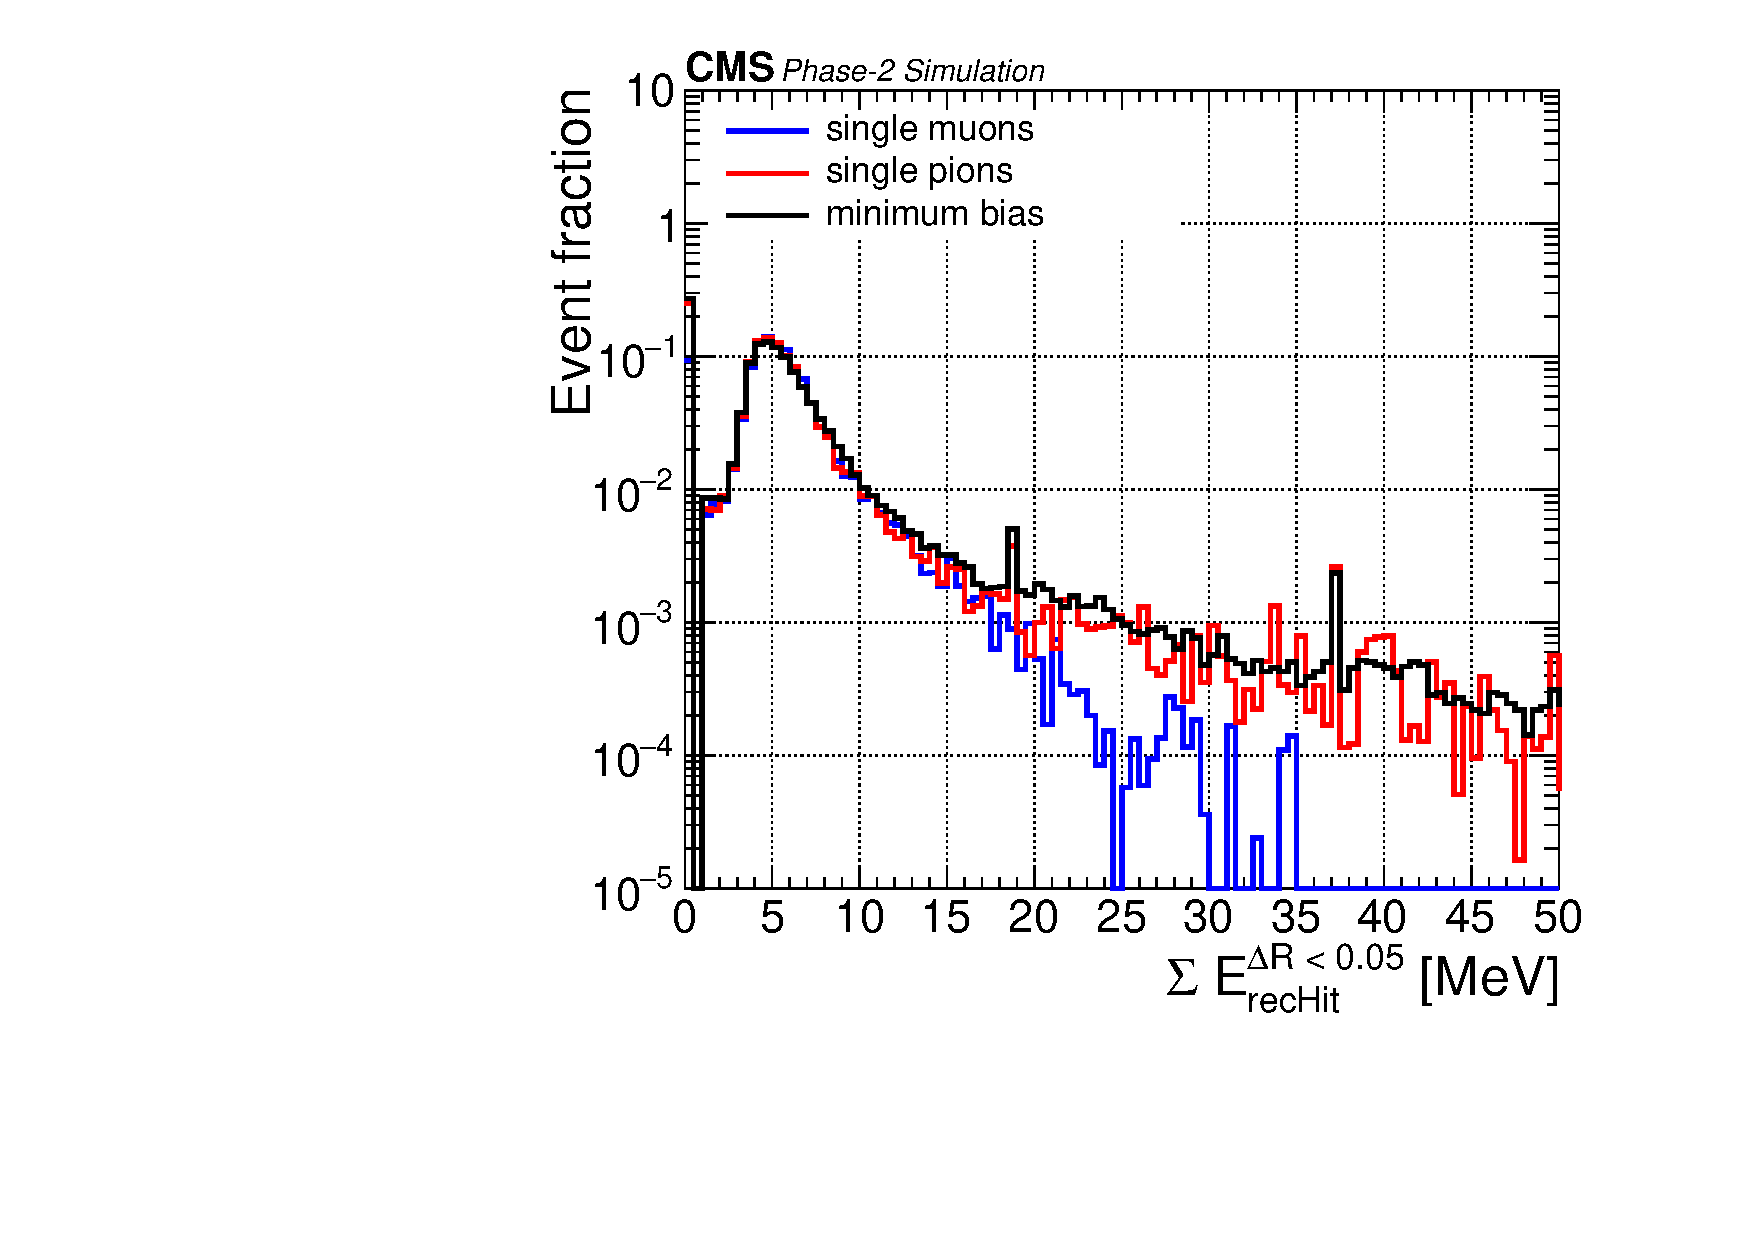
\includegraphics[width=0.49\textwidth]{fig/performance/c_all_Edep.pdf}
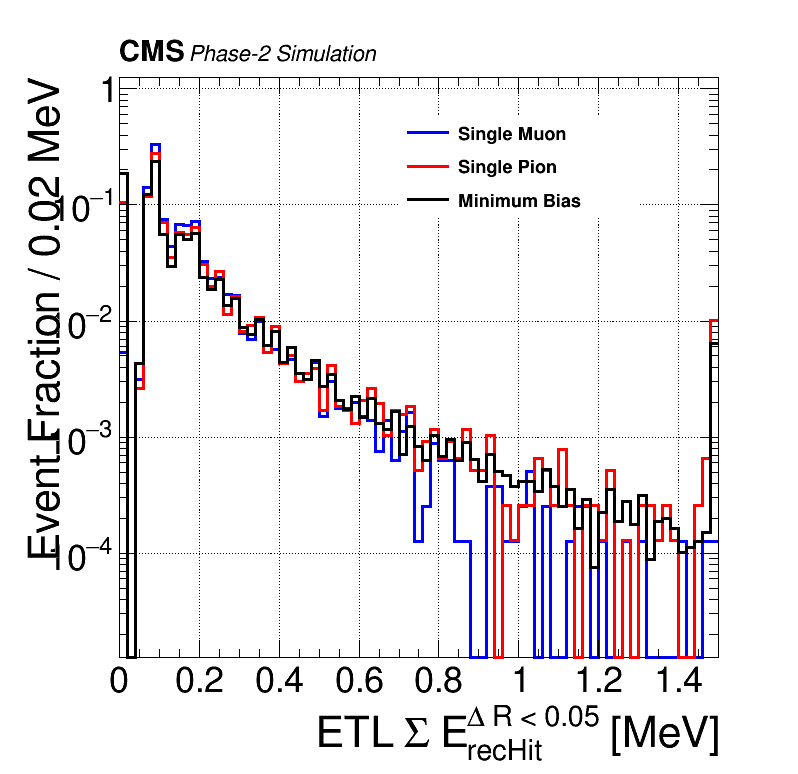
\includegraphics[width=0.45\linewidth]{fig/performance/h_3_recHit_energy_dR05_withTrackETL_20keVbins.png}
%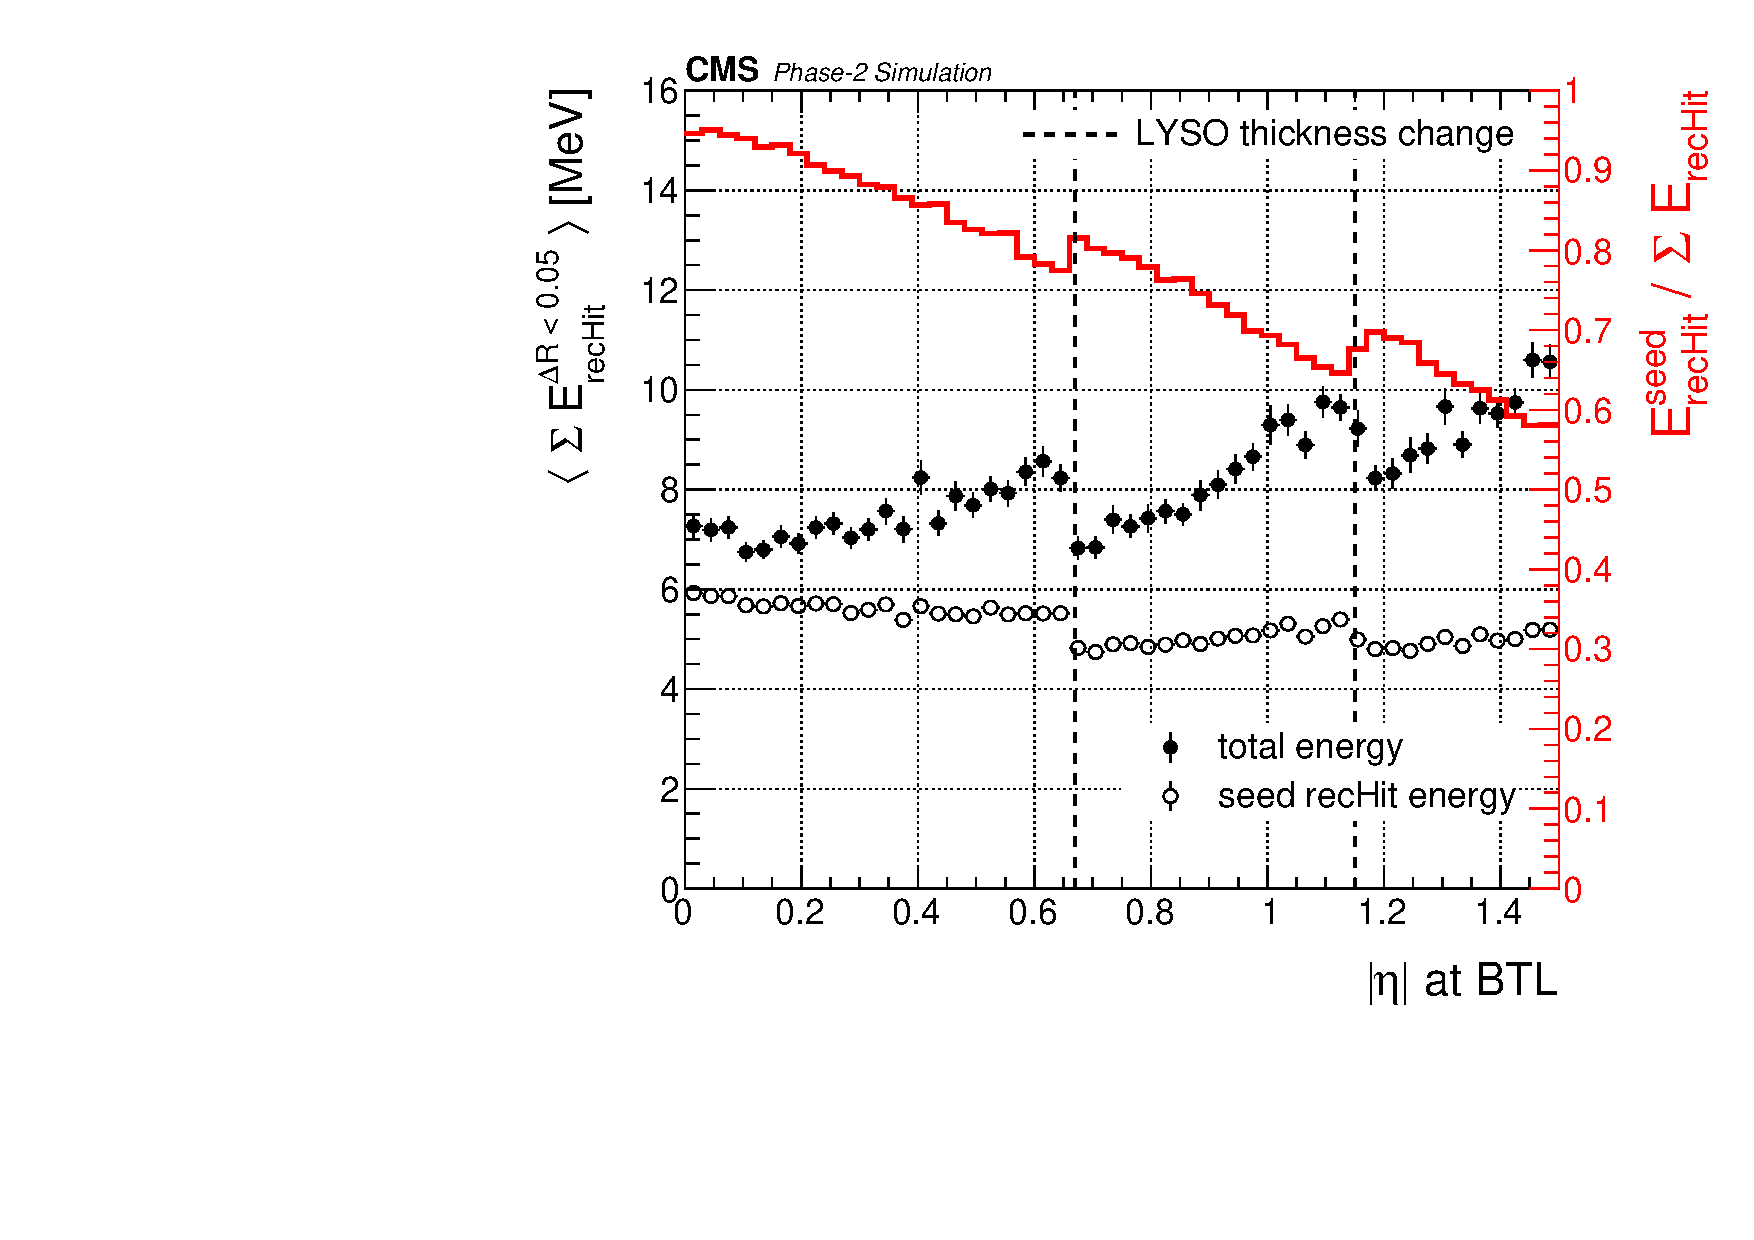
\includegraphics[width=0.48\linewidth]{fig/performance/c_minBias_maxEnergy_vs_eta.pdf}
\caption{Left: Distribution of the energy deposited in the BTL as predicted by the simulation for single muon (blue), single pion (red), and minimum bias events. 
%The energy is reconstructed as the sum of all BTL hits within a cone of $\Delta R < 0.05$ around the track propagated to the BTL front surface. 
Right: Distribution of the energy deposited in the ETL as predicted by the simulation for single muon (blue) and single pions (red). 
%The energy is reconstructed as the sum of all BTL hits within a cone of $\Delta R < 0.05$ around the track propagated to the BTL front surface. 
%on the left and minimum bias events on the right. 
In these plots, single muon and single pion events are weighted so that their $p_{T}$ and $\eta$ spectra match the ones observed for minimum bias events. 
}
%%%PM we probably need to explain the spikes which corresponds to saturation of the electronics 
\label{fig:BTL_Edep}
\end{figure}

%in the upstream material and in BTL itself [TBC]. 
The energy deposition is also shown as a function of the pseudo-rapidity for the BTL in Fig.~\ref{fig:BTL_EdepVsEta_timeRes}-left. 
This figure shows the average total energy deposited by a muon, as well as the average energy deposited in the crystal with highest energy in each cluster (``seed crystal'') and the ratio of these two quantities as a function of pseudorapidity. 
%for single muon and minimum bias events, respectively. 
The energy deposition is fairly independent as a function of $\eta$, because of the crystal slant-thickness leveling. The fraction of energy deposited in the seed crystal, shown in the same plot,  decreases as a function of $|\eta|$ to about 60\% at the end of the barrel, where tracks are more likely to cross adjacent crystals. The energy deposition is also fairly uniform in ETL, since the sensors remain the same thickness throughout the annulus covered by the detector, driven by the need to keep the
depleted region of the silicon sensors thin to reduce the impact of
Landau fluctuations on the sensor's timing resolution.
%The effect of crystal thickness leveling in three pseudorapidity regions reflects in the equalization of the average total energy deposit along $\eta$. 
%Because of the crystal arrangement, inclined tracks at high $\eta$ are likely to cross multiple adjacent crystals, so that the fraction of energy deposited in the most energetic of them decreases, on average, to about 60\% at the end of the barrel.

\begin{figure}[hbtp]
\centering
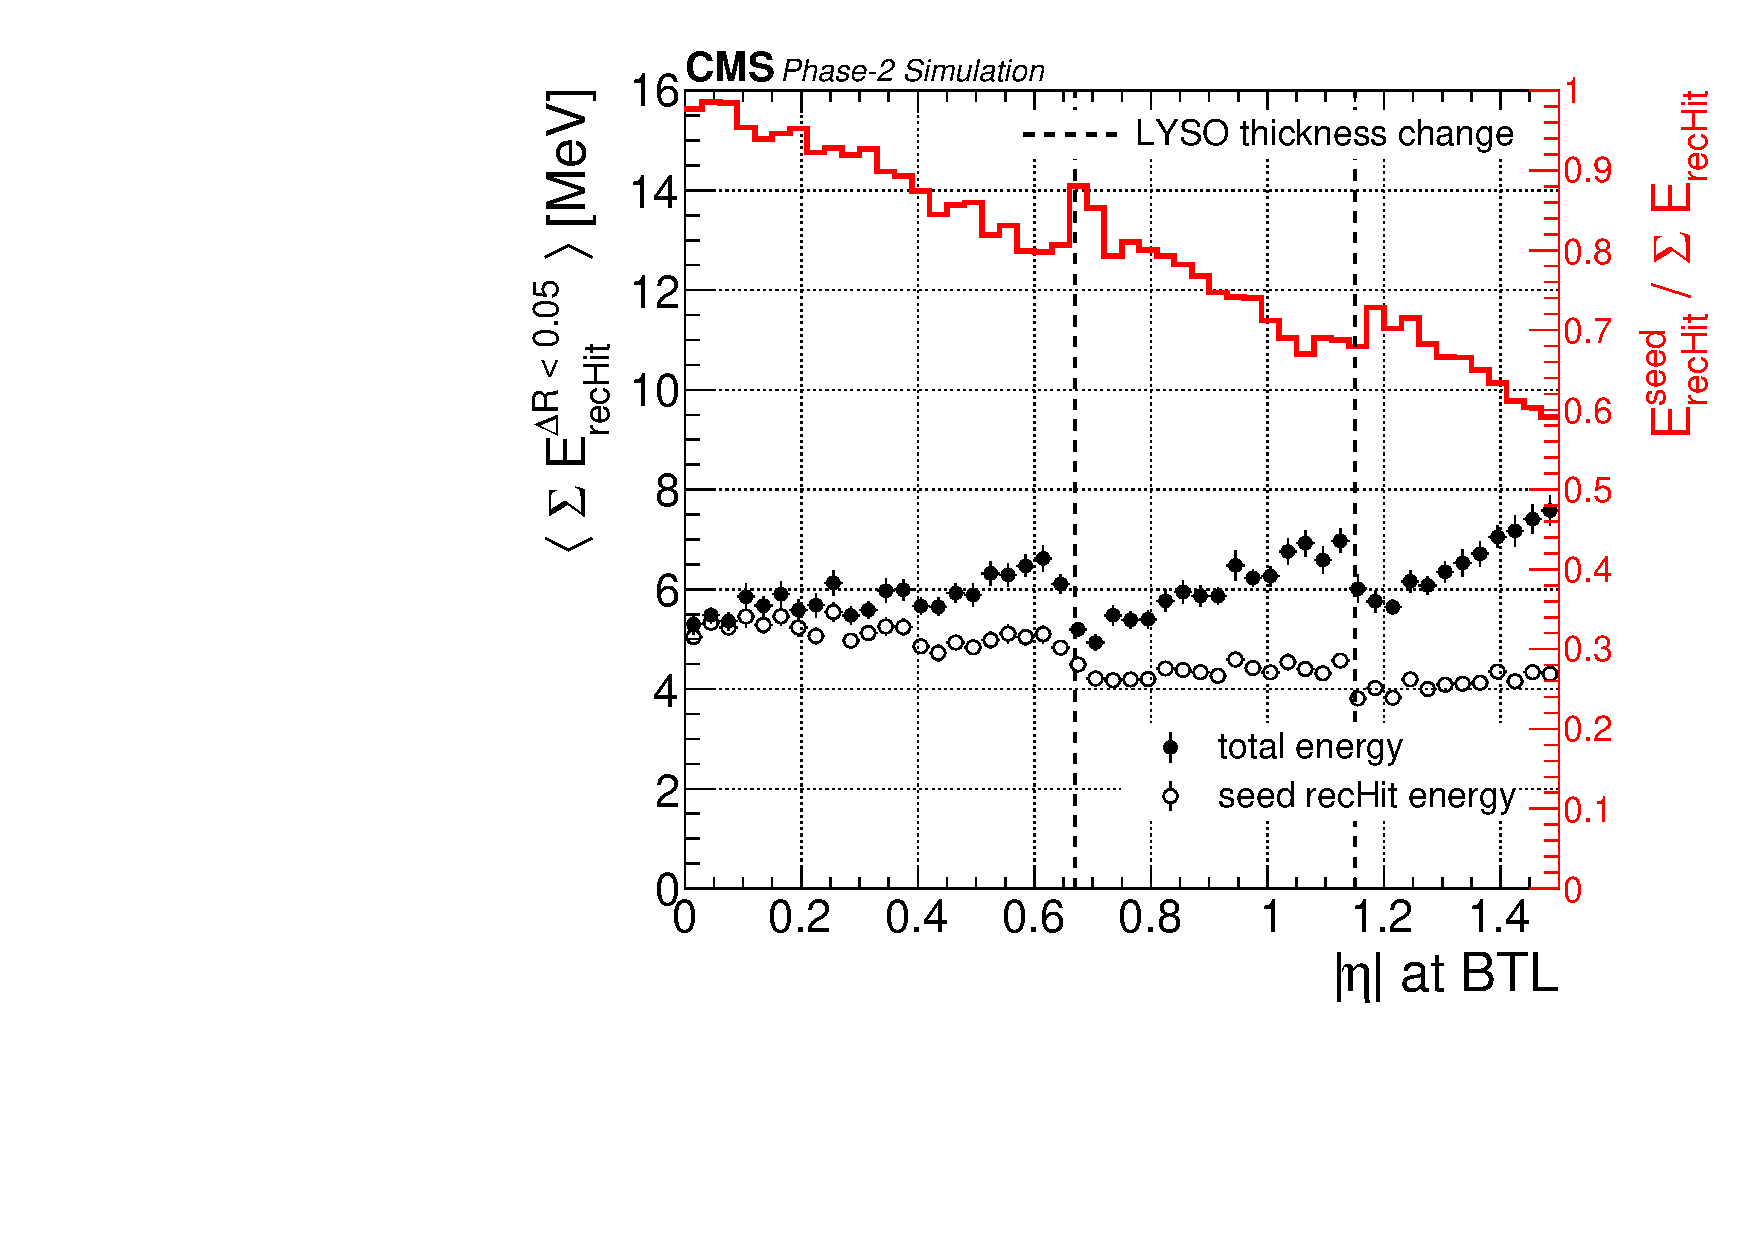
\includegraphics[width=0.49\linewidth]{fig/performance/c_singleMuPtFlat_maxEnergy_vs_eta.pdf}
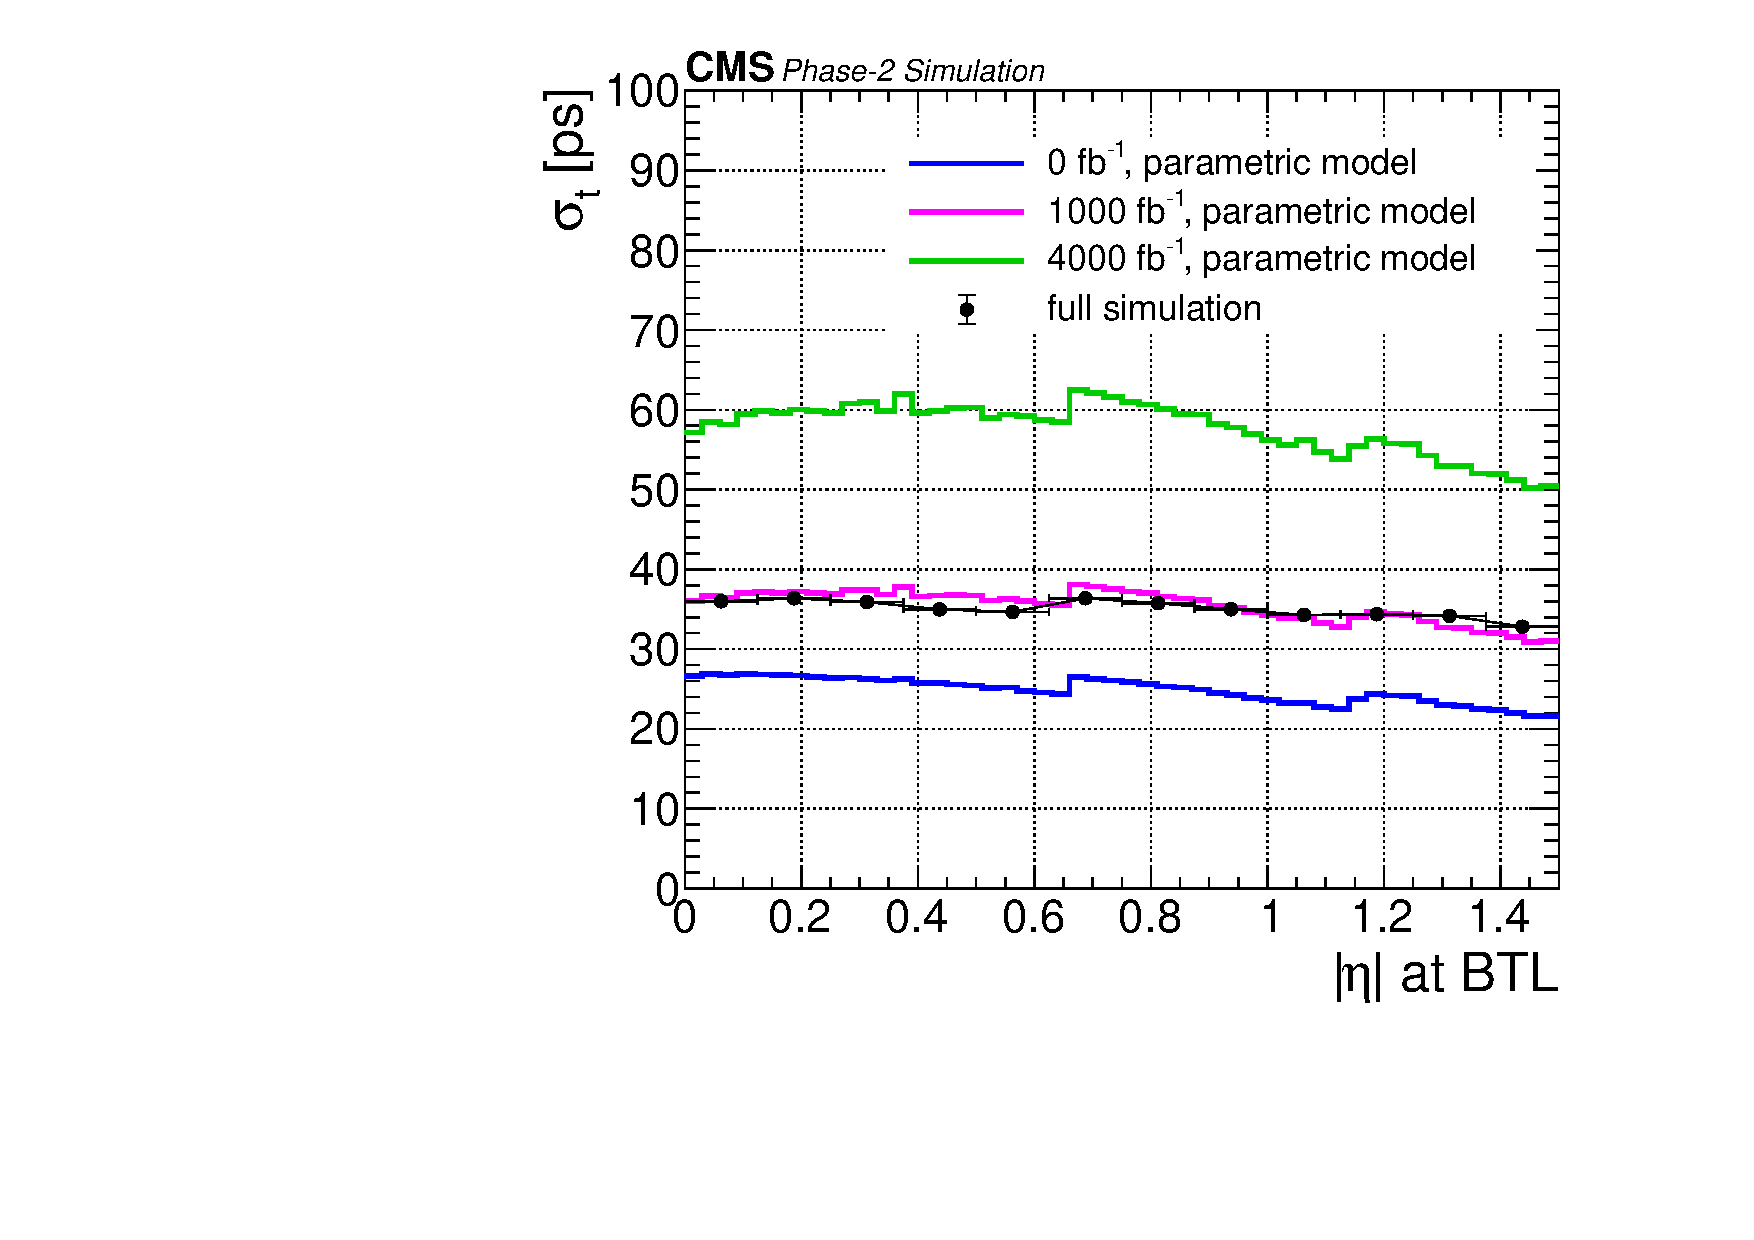
\includegraphics[width=0.49\textwidth]{fig/performance/c_MinBias_timeRes_vs_eta.pdf}
\caption{Left: Average total energy deposit (black solid dots), energy of the seed crystal (empty dots) and ratio of the two above quantities (red line, right axis) as a function of pseudorapidity, for single muon events. Right: Average time resolution for clusters associated to tracks in minimum bias events for three ageing scenarios corresponding to 0 (blue), 1000 (purple), and 4000~fb$^{-1}$ (green). The prediction of the parametric model compared to the full simulation for 1000 fb$^-1$.
}
%%%PM we probably need to explain the spikes which corresponds to saturation of the electronics 
\label{fig:BTL_EdepVsEta_timeRes}
\end{figure}

%[Discuss amplitude walk correction here?]

%[Text taken from 2.1.1.1]

The time measurement associated to a cluster is obtained
from the average of single-hits time measurements, weighted on the
respective resolutions.  In BTL the time measurement for a single crystal is
obtained from a linear combination of the left and the right SiPMs
measurements, $t_{\text{ave}} = C_{L} \cdot t_{L} + C_{R} \cdot t_{R }$; where $C_{L}$
and $C_{R}$ are two calibration coefficients that can be  
derived in situ. According to test beam results for particles at
normal incidence (Section~2.1.1), the time measurement is independent
of the track impact point along the crystal for $C_{L} = C_{R} = 0.5$.  
These values are adopted in the current simulation and in the studies
reported in the TDR.  

The expected average time resolution for clusters associated to
tracks in minimum bias events is shown for BTL Fig.~\ref{fig:BTL_EdepVsEta_timeRes}-right 
for three ageing scenarios corresponding to 0, 1000, and
4000~fb$^{-1}$. The response evolution is parameterized according
to the model described in Section~2.1, normalized to test beam 
results by means of a \GEANT simulation of the test beam setup. 

%
%The energy distribution profiles of Fig.~\ref{fig:BTL_Edep} allow the performance of the BTL in time reconstruction to be predicted as a function of the pseudorapidity, as shown in Fig.~\ref{fig:BTL_timeRes} for three different aging scenarios corresponding to 0, 1000, and 4000~fb$^{-1}$. The single sensor timing resolution for the unaged detector and a 2.6 MeV most probable energy deposit in one crystal is assumed to be 43 ps, as measured in beam tests. This number is then scaled by the actual energy deposit predicted by the simulation, and other contributions to the timing resolution -- the DCR term being the dominant one -- are added in quadrature, according to the parametric model described in Sec.~2.1. The timing resolution as predicted by the full simulation is also superimposed. In the plots, the timing resolution is shown after combining the individual resolutions expected in each crystal of the cluster.   
%
The average per-track resolution for tracks with the \pt spectrum of 
minimum bias events is \tres or better across the full BTL acceptance up to 
1000~fb$^{-1}$, while it drifts to \trend at the end of  operations.  
The average resolution during the HL-LHC operation (2000 fb$^{-1}$) is 
about 40~ps. The results from the full simulation corresponding to
1000~fb$^{-1}$ are used as a reference for physics studies. 


%\subsubsection{ETL}

%The energy deposited by a particle in the ETL is reconstructed adding
%all the information of all cells above the readout threshold that lie
%within a cone of $\Delta R = 0.03$ around the extrapolation of track
%to the ETL surface. 
%[NB: As with BTL, this description is valid for the current plots. Text and the plots need to be updated to reflect
%the usage of clusters].  
%The distribution of the total energy deposit
%predicted by the full simulation of single muon, single pion and
%minimum bias events is reported in the top panel of
%Fig.~\ref{fig:ETL_Edep}. Muons behave as MIP in the timing layer, and
%their most  probable and average energy deposit correspond to about X
%and Y.Y MeV, respectively. Hadrons, instead, show a larger total
%energy deposit of about Z MeV due to high energy tails from
%interactions  in the tracker. The average total energy deposit in ETL,
%as well as the average energy deposited in the seed pad of each ETL
%cluster and the ratio of these two quantities, are reported in the
%central and bottom panels of Fig.~\ref{fig:ETL_Edep} as a function of
%pseudorapidity, for single muon and minimum bias events,
%respectively..

%\begin{figure}[hbtp]
%\centering
%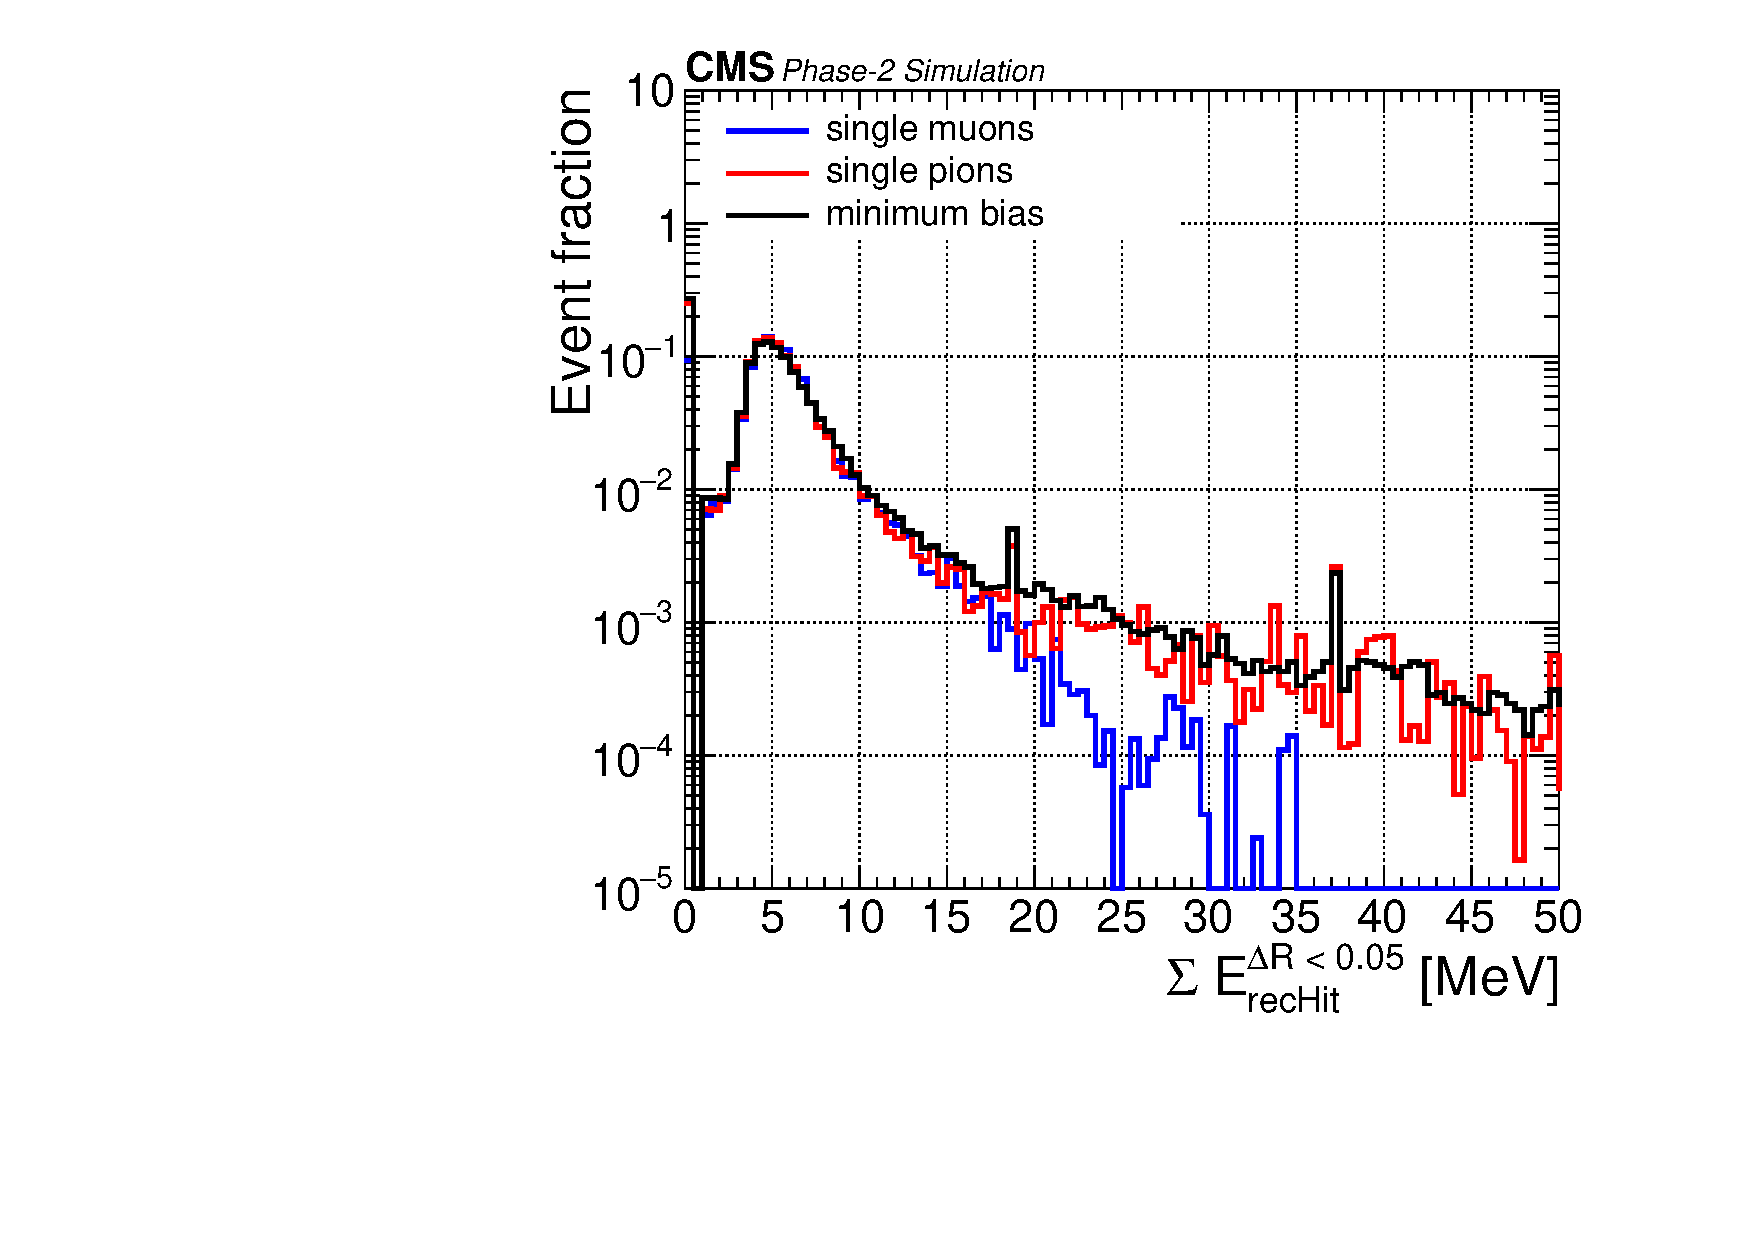
\includegraphics[width=0.48\textwidth]{fig/performance/c_all_Edep.pdf}
%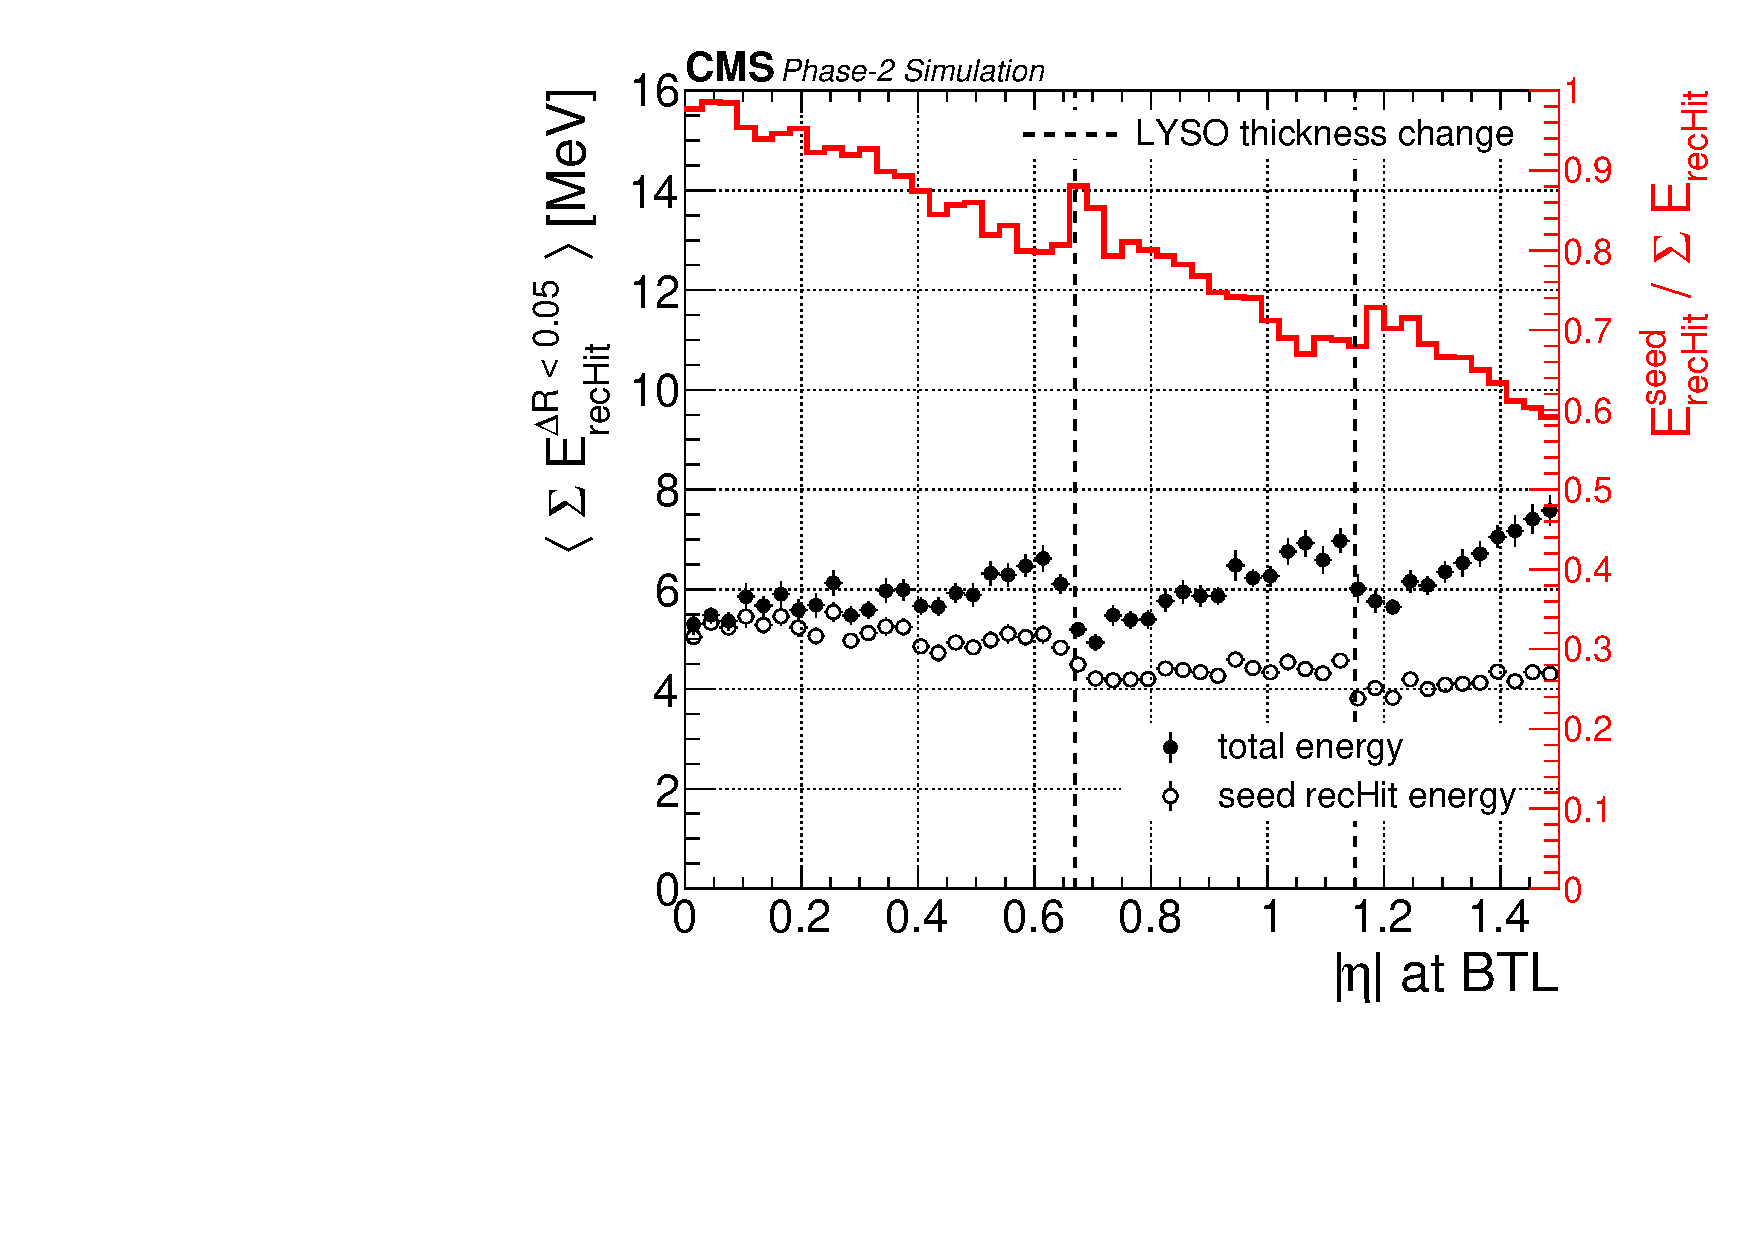
\includegraphics[width=0.48\linewidth]{fig/performance/c_singleMuPtFlat_maxEnergy_vs_eta.pdf}
%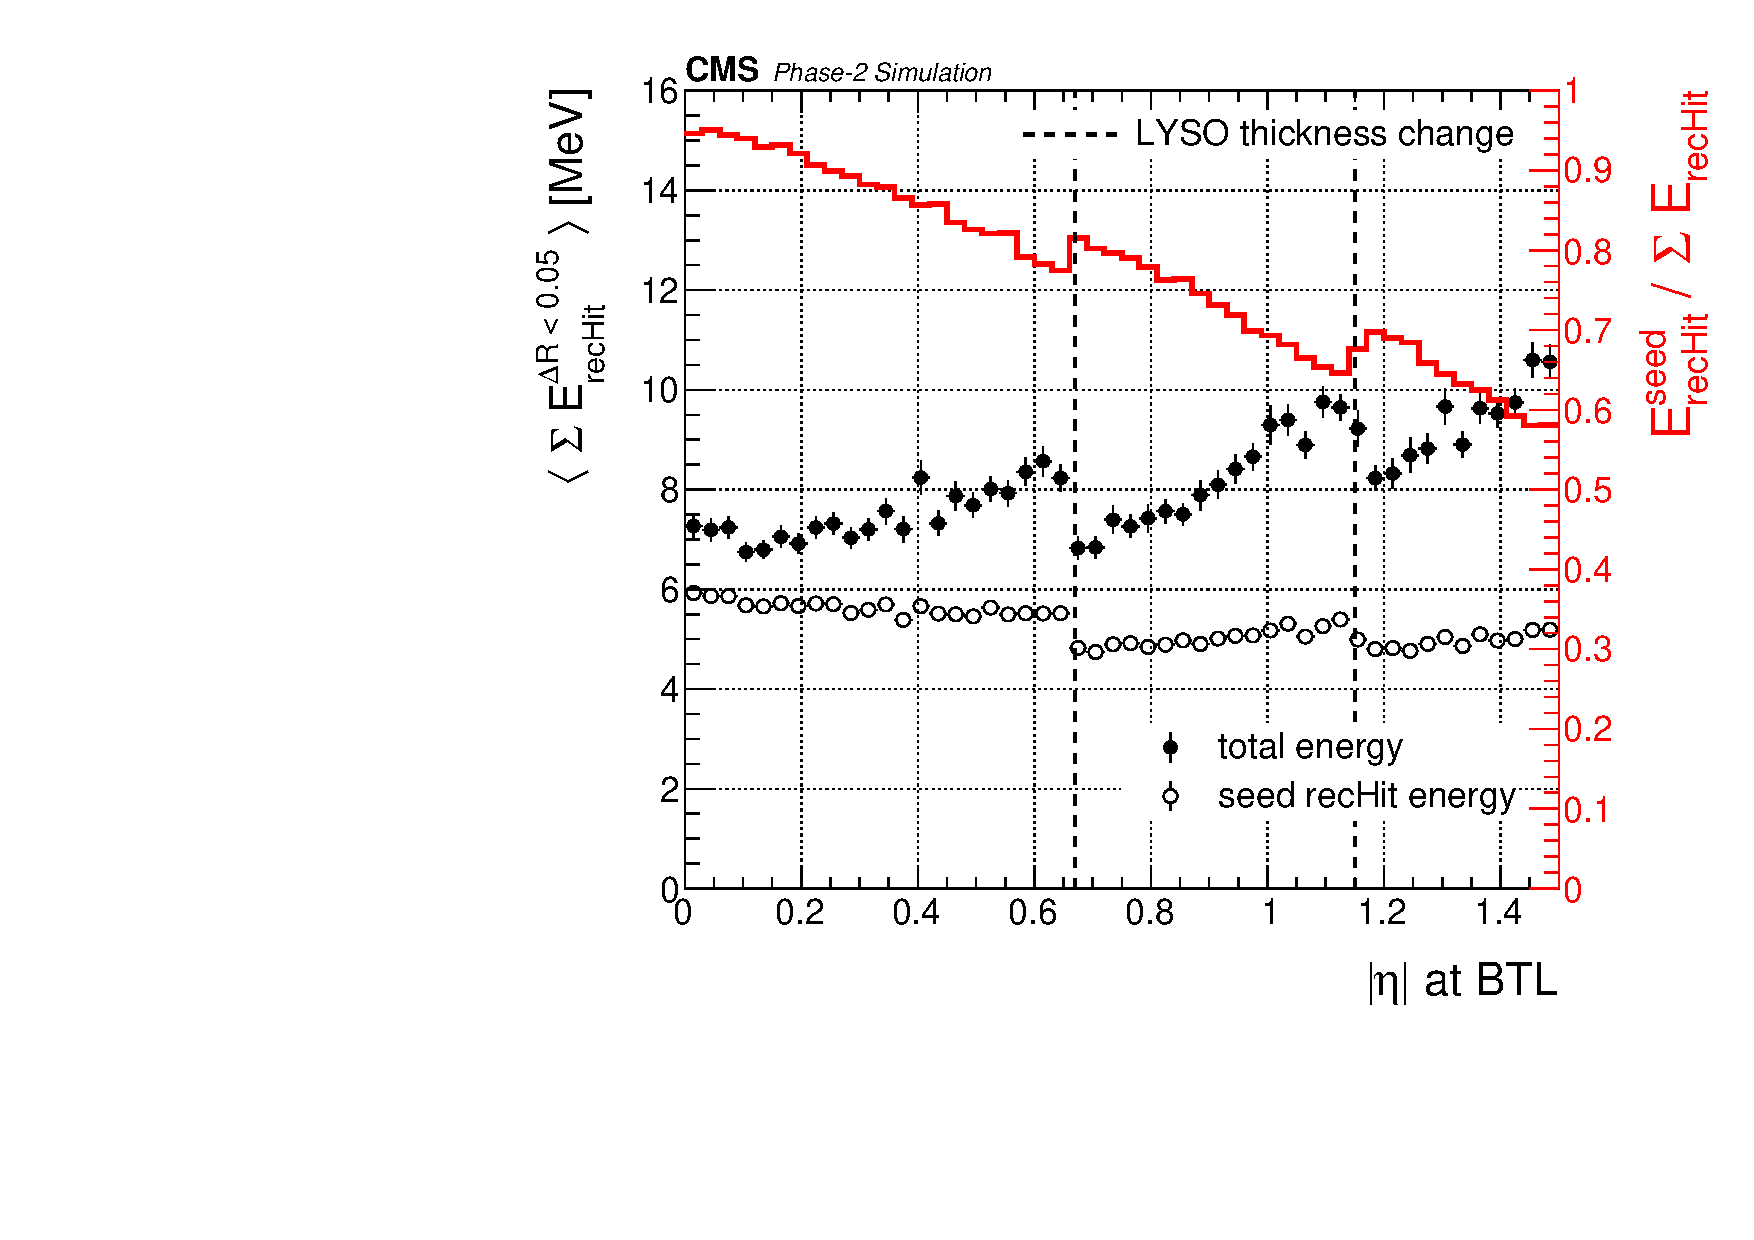
\includegraphics[width=0.55\linewidth]{fig/performance/c_minBias_maxEnergy_vs_eta.pdf}
%\caption{FIXME - ETL PLOTS Left: distribution of the energy deposited in the ETL as predicted by the simulation for single muon (blue), single pion (red), and minimum bias events. The energy is reconstructed as the sum of all ETL hits within a cone of $\Delta R < 0.02$ around the track propagated to the ETL front surface. Right: average total energy deposit (black solid dots), energy of the seed crystal (empty dots) and ratio of the two above quantities (red line, right axis) as a function of pseudorapidity, for single muon events.
%}
%\label{fig:ETL_Edep}
%\end{figure}

%Given the less advanced state of the electronics studies for ETL at the time of developing its simulation chain, the digitization routine for this detector is simpified to be a smearing of a threshold crossing time of simulated hits in each ETL pad with a threshold of 0.02 of the average energy deposition of a MIP in the LGAD's depleted region. The injected time resolution is 35~ps. The ETL local reconstruction accounts for the conversion of the digitizer output into hits with recorded energy and coordinate values, and prepares the hits for use in the tracking reconstruction described later in this text.

%%%PM Energy deposition for single mu, single pi and minimum bias
%%%PM Time resolution can be just a sentence given that there is just a simple smearing

\section{Clustering}

%editors: L. Gray & P. Meridiani
In the first step of the MTD track reconstruction, a simple topological clustering is performed to associate adjacent MTD hits above the readout threshold. 
%In particular, multiple hits can be associated to a single track which impacts BTL at a shallow angle, either at p$_{T}$ below 2\mathrm{GeV} or at higher pseudo-rapidity values (above $|\eta|>0.8$). 
Hits are required to be compatible in time, as this shows to mildly improve the resolution of the cluster parameters at high pile-up. The baricenter, weighted by the single hit energy, is used as an estimate of the cluster position and time. 

Comparison of the cluster size and reconstructed time 
%and the cluster reconstructed position 
is shown in Figure \ref{fig:clusterMuPuComp_BTL} and \ref{fig:clusterMuPuComp_ETL} for single muon simulated events with an average of 200 pile-up events and without pile-up for BTL and ETL respectively.

\begin{figure}[!h]
\centering
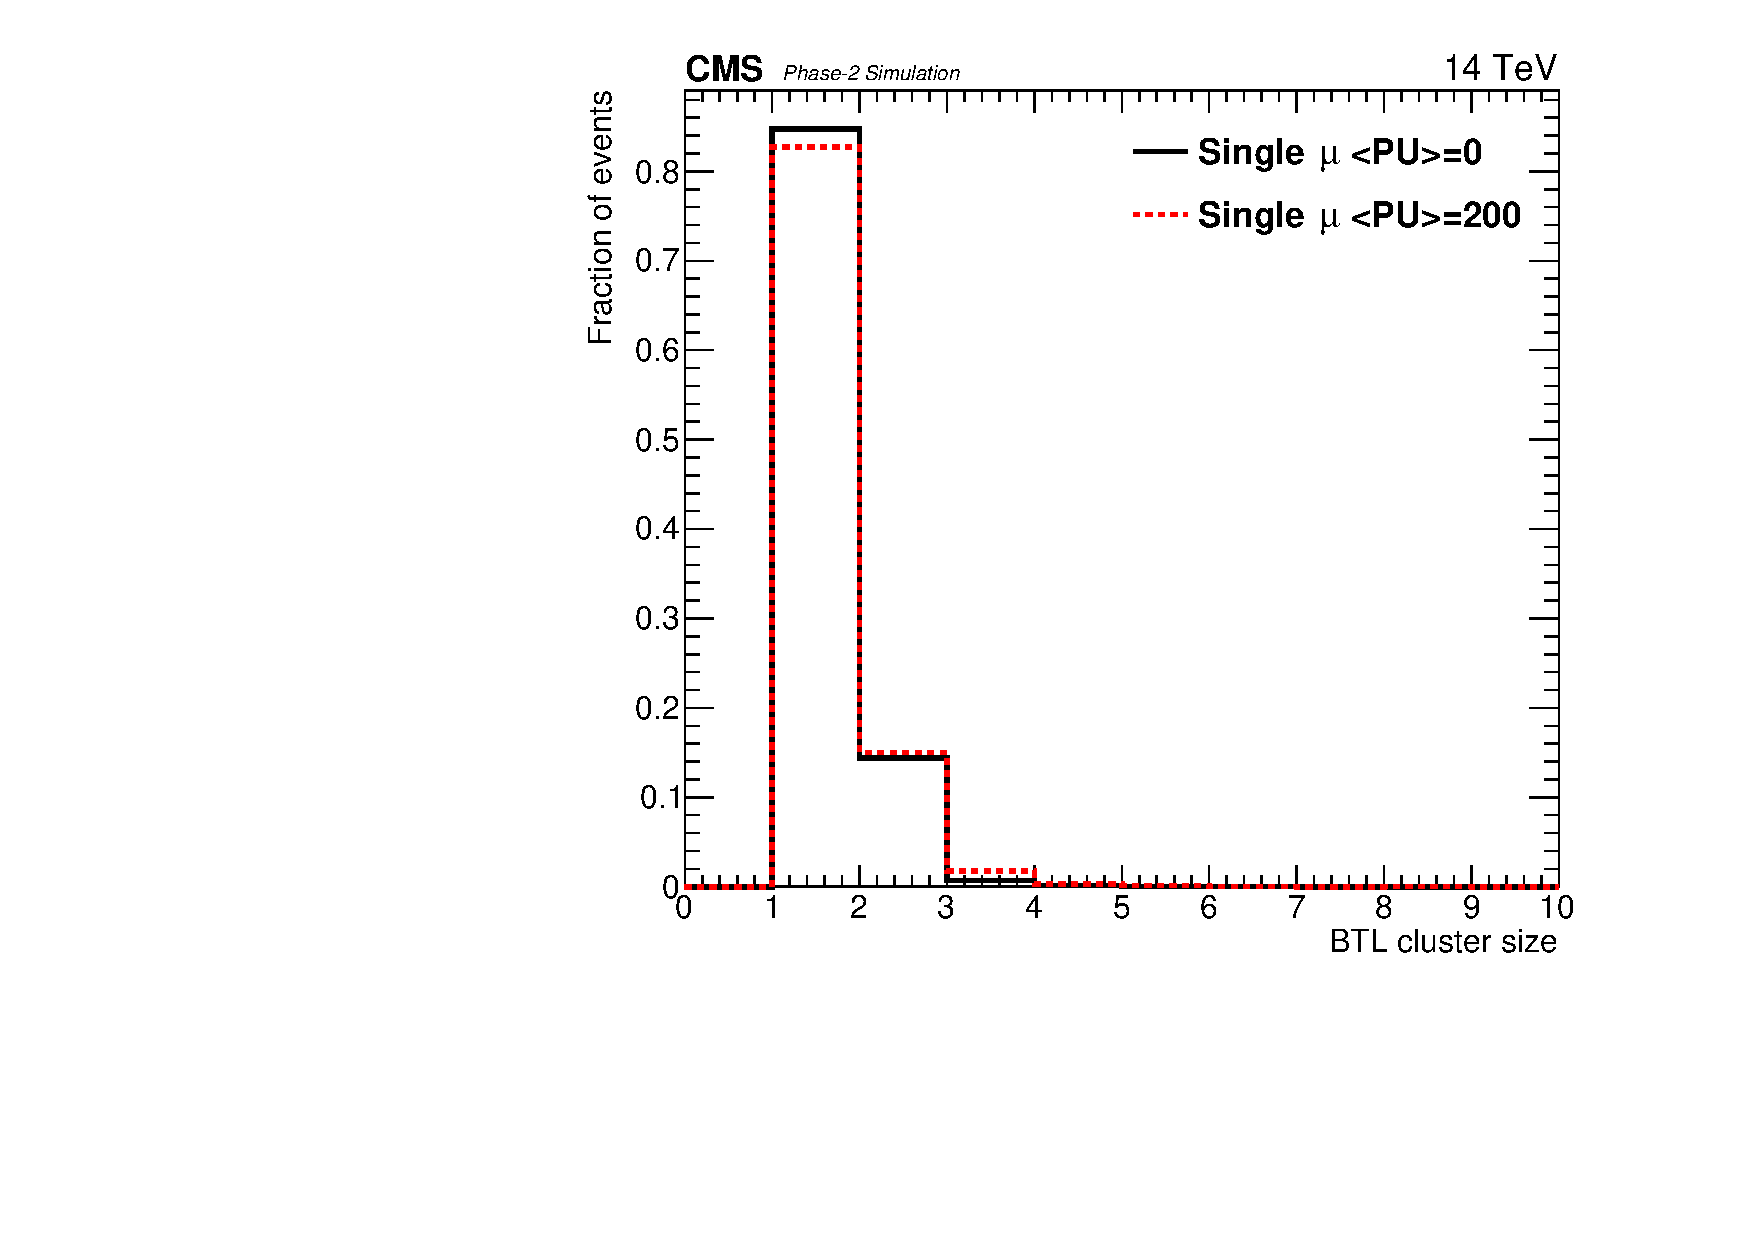
\includegraphics[width=0.48\textwidth]{fig/performance/ClusterAndTracks/noPreliminary/BTLbestCluster_size_muPUcomp-4.pdf}
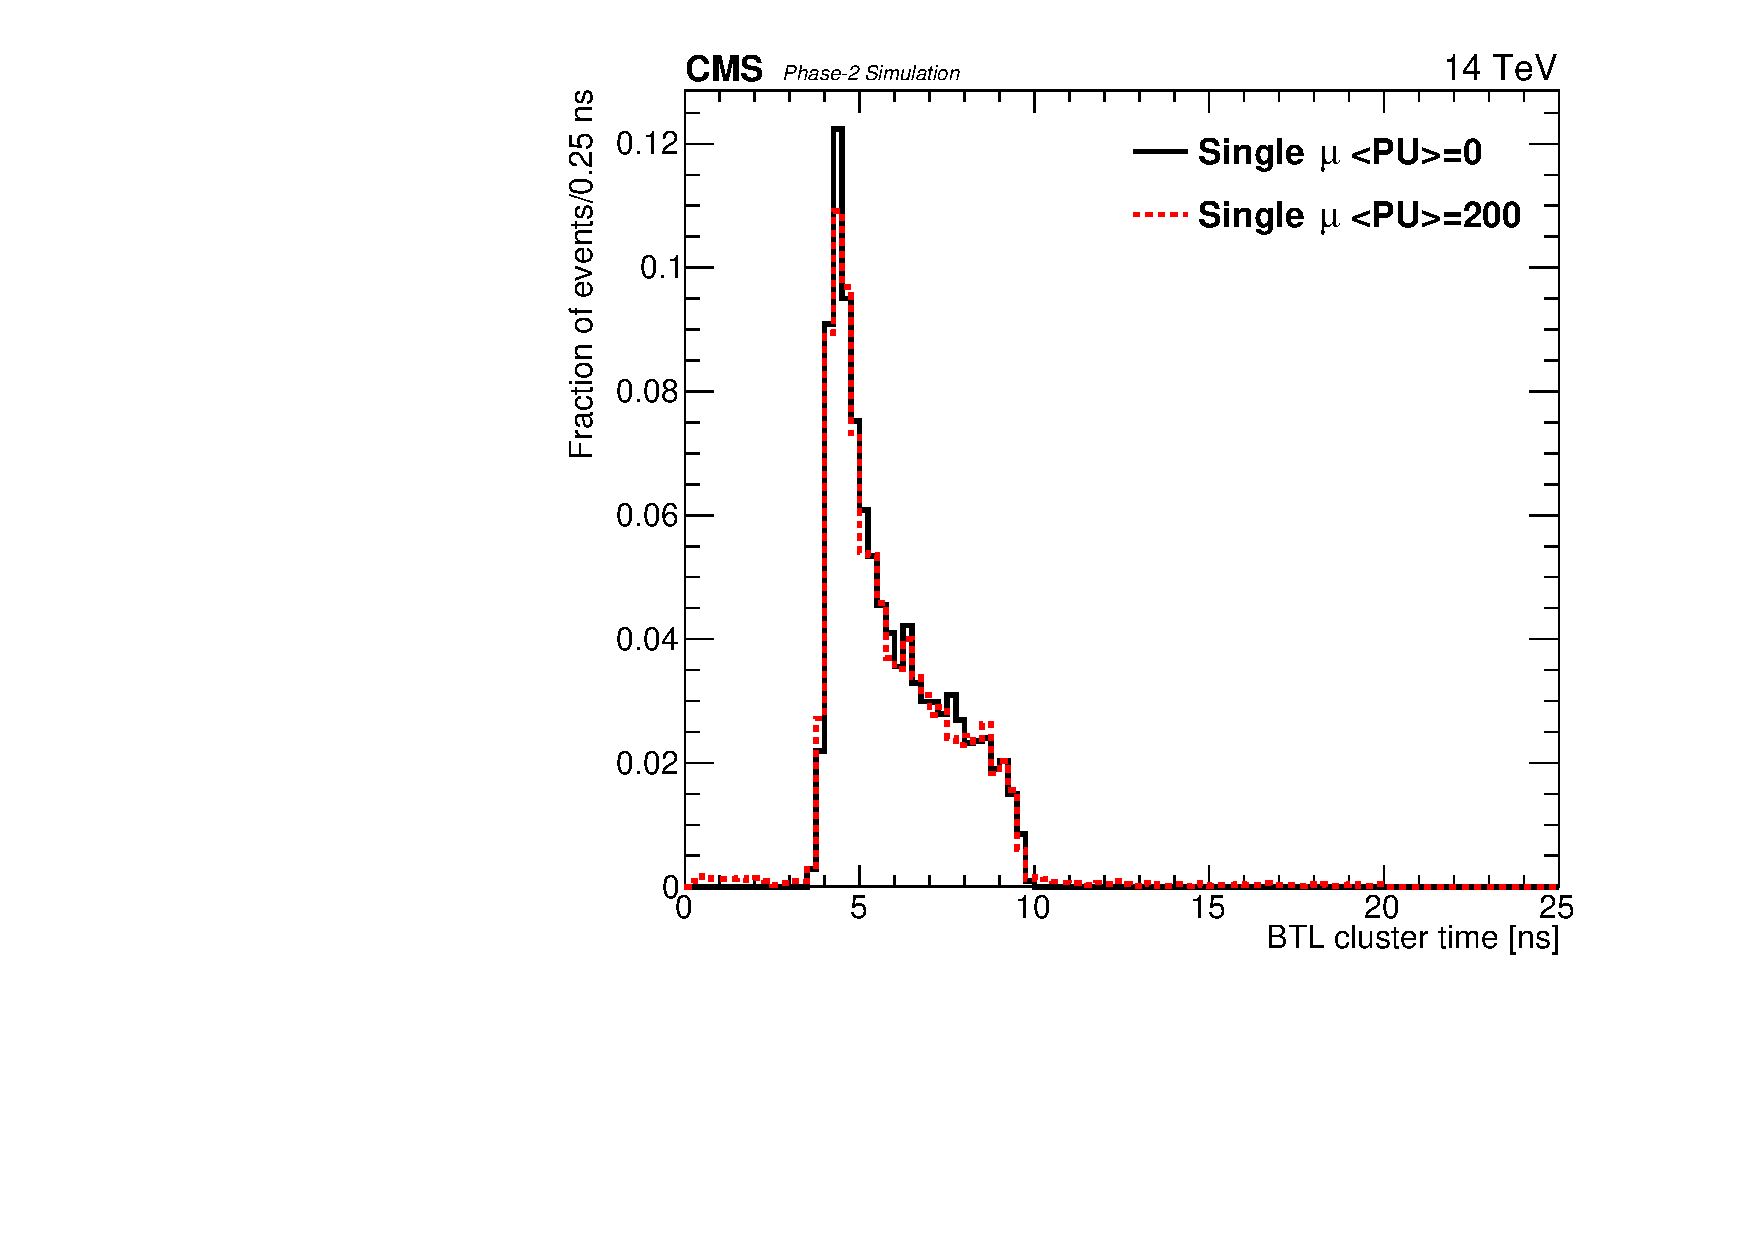
\includegraphics[width=0.48\textwidth]{fig/performance/ClusterAndTracks/noPreliminary/BTLbestCluster_time_muPUcomp-4.pdf}
%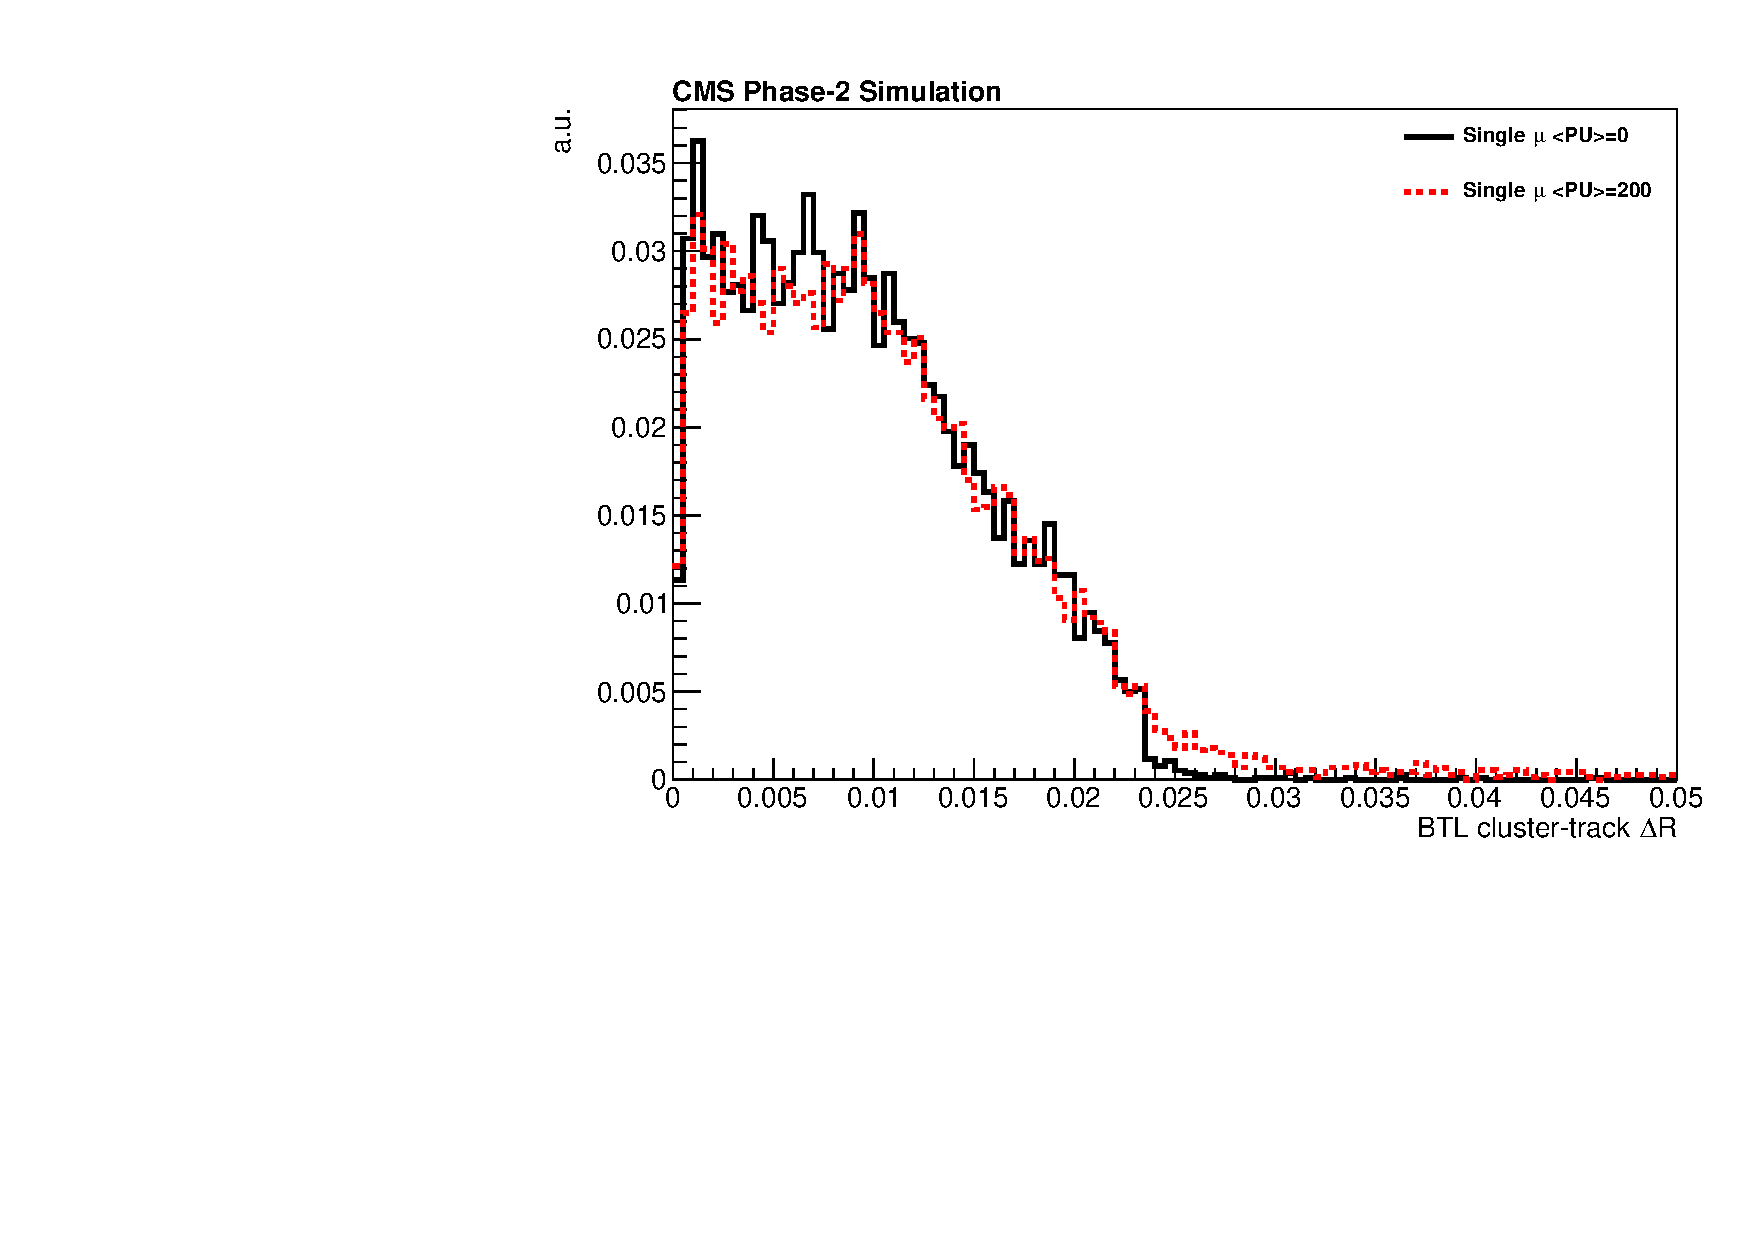
\includegraphics[width=0.32\textwidth]{fig/performance/ClusterAndTracks/BTLbestCluster_DR_muPUcomp.pdf}
\caption{Comparison of the BTL clusters size (left) and reconstructed time (right)
%and $\Delta R$ between the track propagated at the MTD and the cluster position
for single muon events (flat $p_{T}$ spectrum in 0.7-10~GeV range) with an average of 200 pile-up events(red dotted line) and without pile-up (black line).}
\label{fig:clusterMuPuComp_BTL}
\end{figure}

\begin{figure}[!h]
\centering
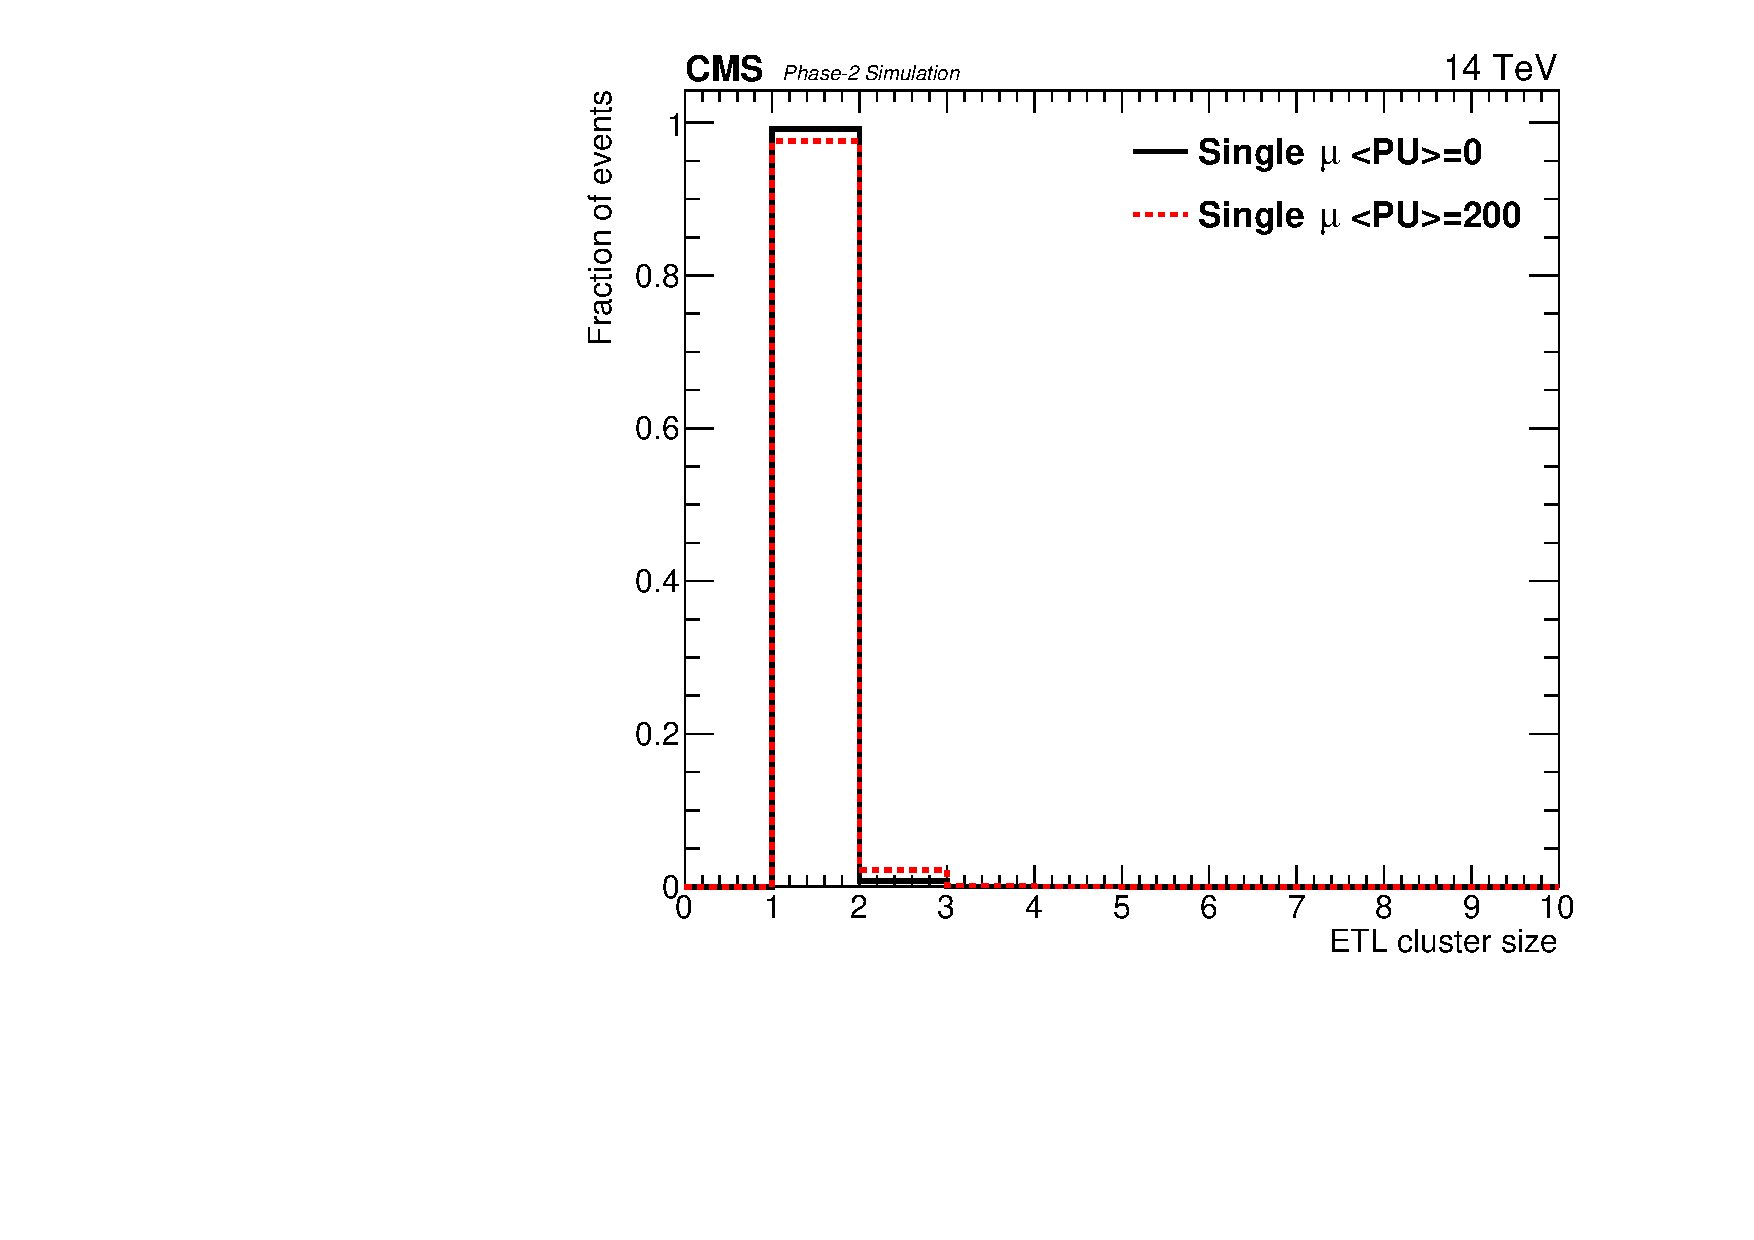
\includegraphics[width=0.48\textwidth]{fig/performance/ClusterAndTracks/noPreliminary/ETLbestCluster_size_muPUcomp-4.pdf}
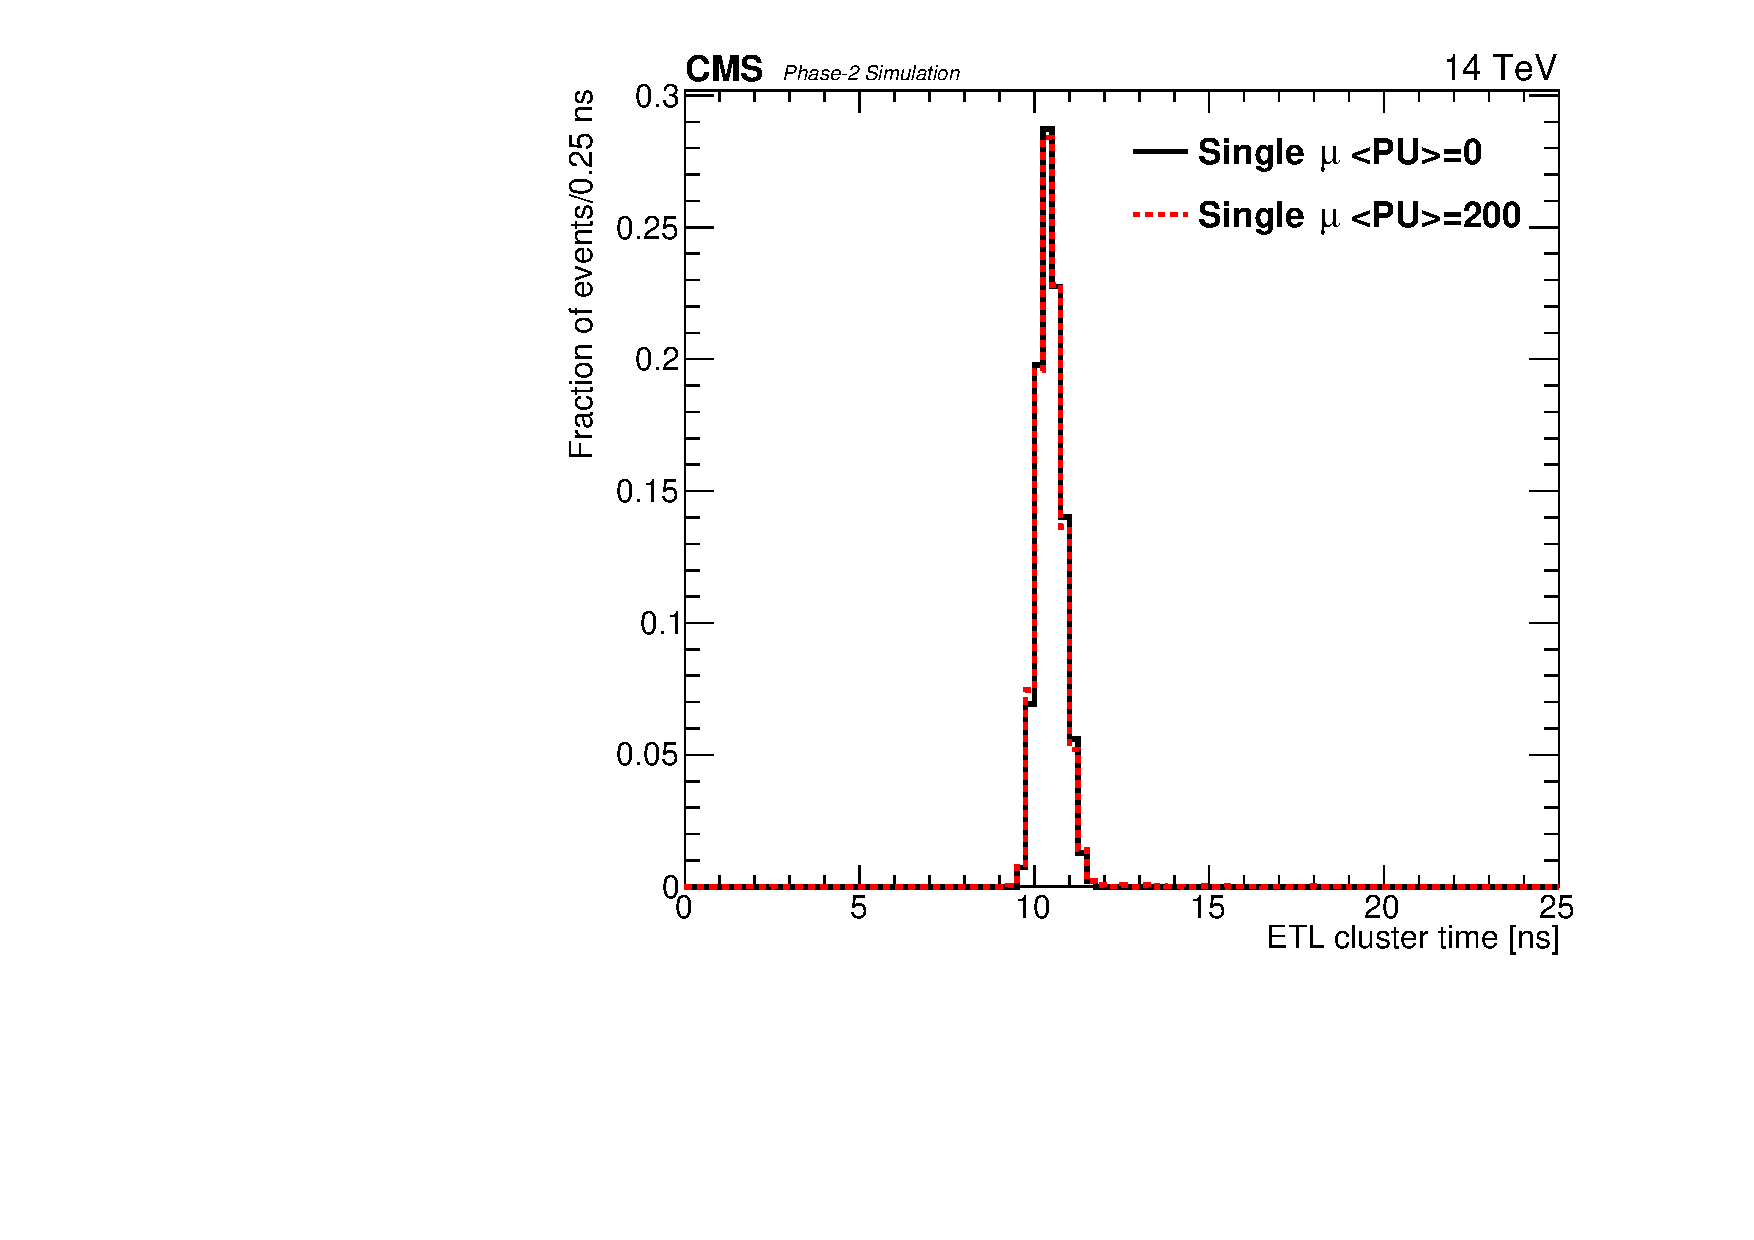
\includegraphics[width=0.48\textwidth]{fig/performance/ClusterAndTracks/noPreliminary/ETLbestCluster_time_muPUcomp-4.pdf}
%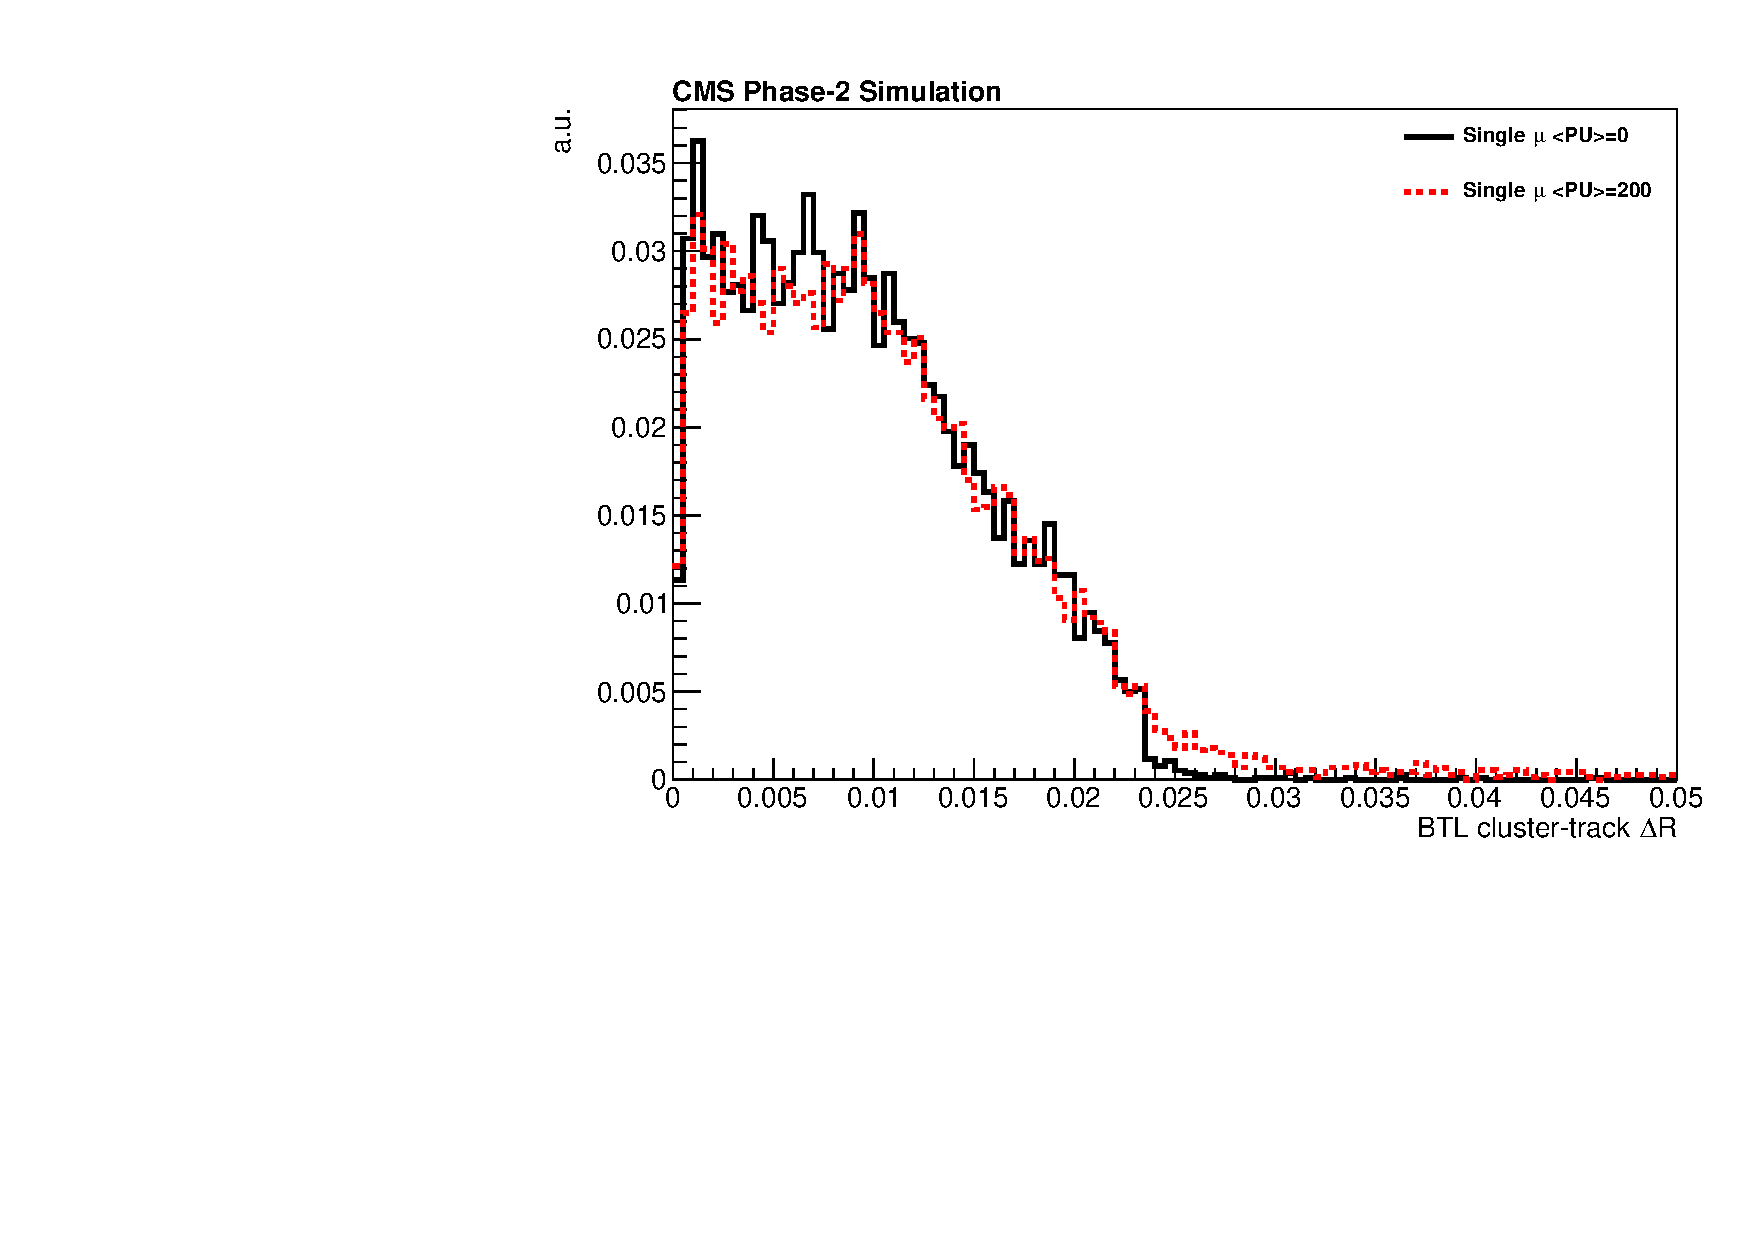
\includegraphics[width=0.32\textwidth]{fig/performance/ClusterAndTracks/BTLbestCluster_DR_muPUcomp.pdf}
\caption{Comparison of the ETL clusters size (left) and reconstructed time (right)
%and $\Delta R$ between the track propagated at the MTD and the cluster position
for single muon events (flat $p_{T}$ spectrum in 0.7-10~GeV range) with an average of 200 pile-up events(red dotted line) and without pile-up (black line).}
\label{fig:clusterMuPuComp_ETL}
\end{figure}

The $\Delta R$ of the best matching cluster in BTL and ETL is shown in Fig.~\ref{fig:clusterMuPuComp_DeltaR} for single muon events with PU200 and without pile-up.
The $\Delta R$ matching precision in the BTL is dominated by the uncertainty in the longitudinal direction of the LYSO bar. The possibility to measure the position along the longitudinal direction of the bar from the difference of the two time readings at the opposite ends of the bar is not yet exploited to compute the cluster position, but it will bring a significant improvement to the matching precision (the impact point longitudinal position resolution on a single bar is estimated to be below 5mm). 

\begin{figure}[!h]
\centering
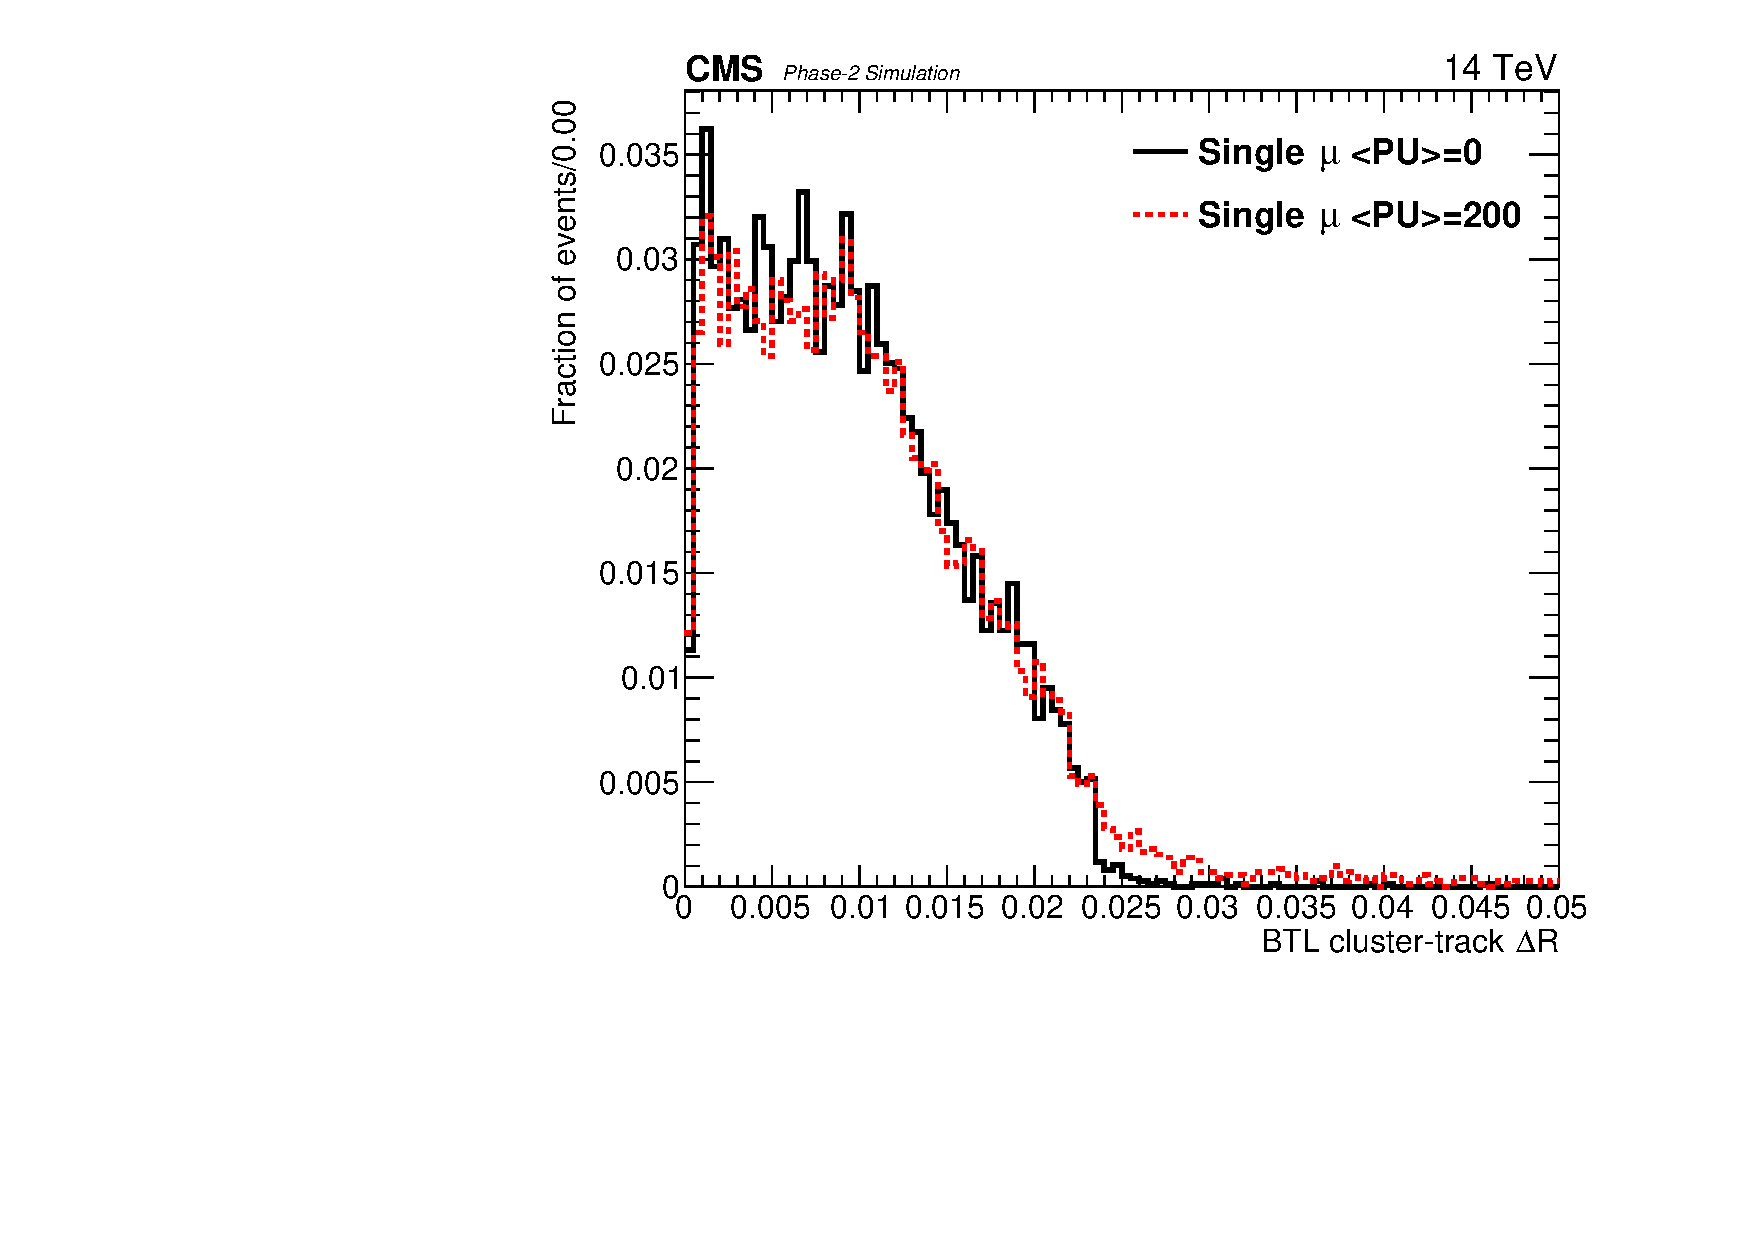
\includegraphics[width=0.48\textwidth]{fig/performance/ClusterAndTracks/noPreliminary/BTLbestCluster_DR_muPUcomp-4.pdf}
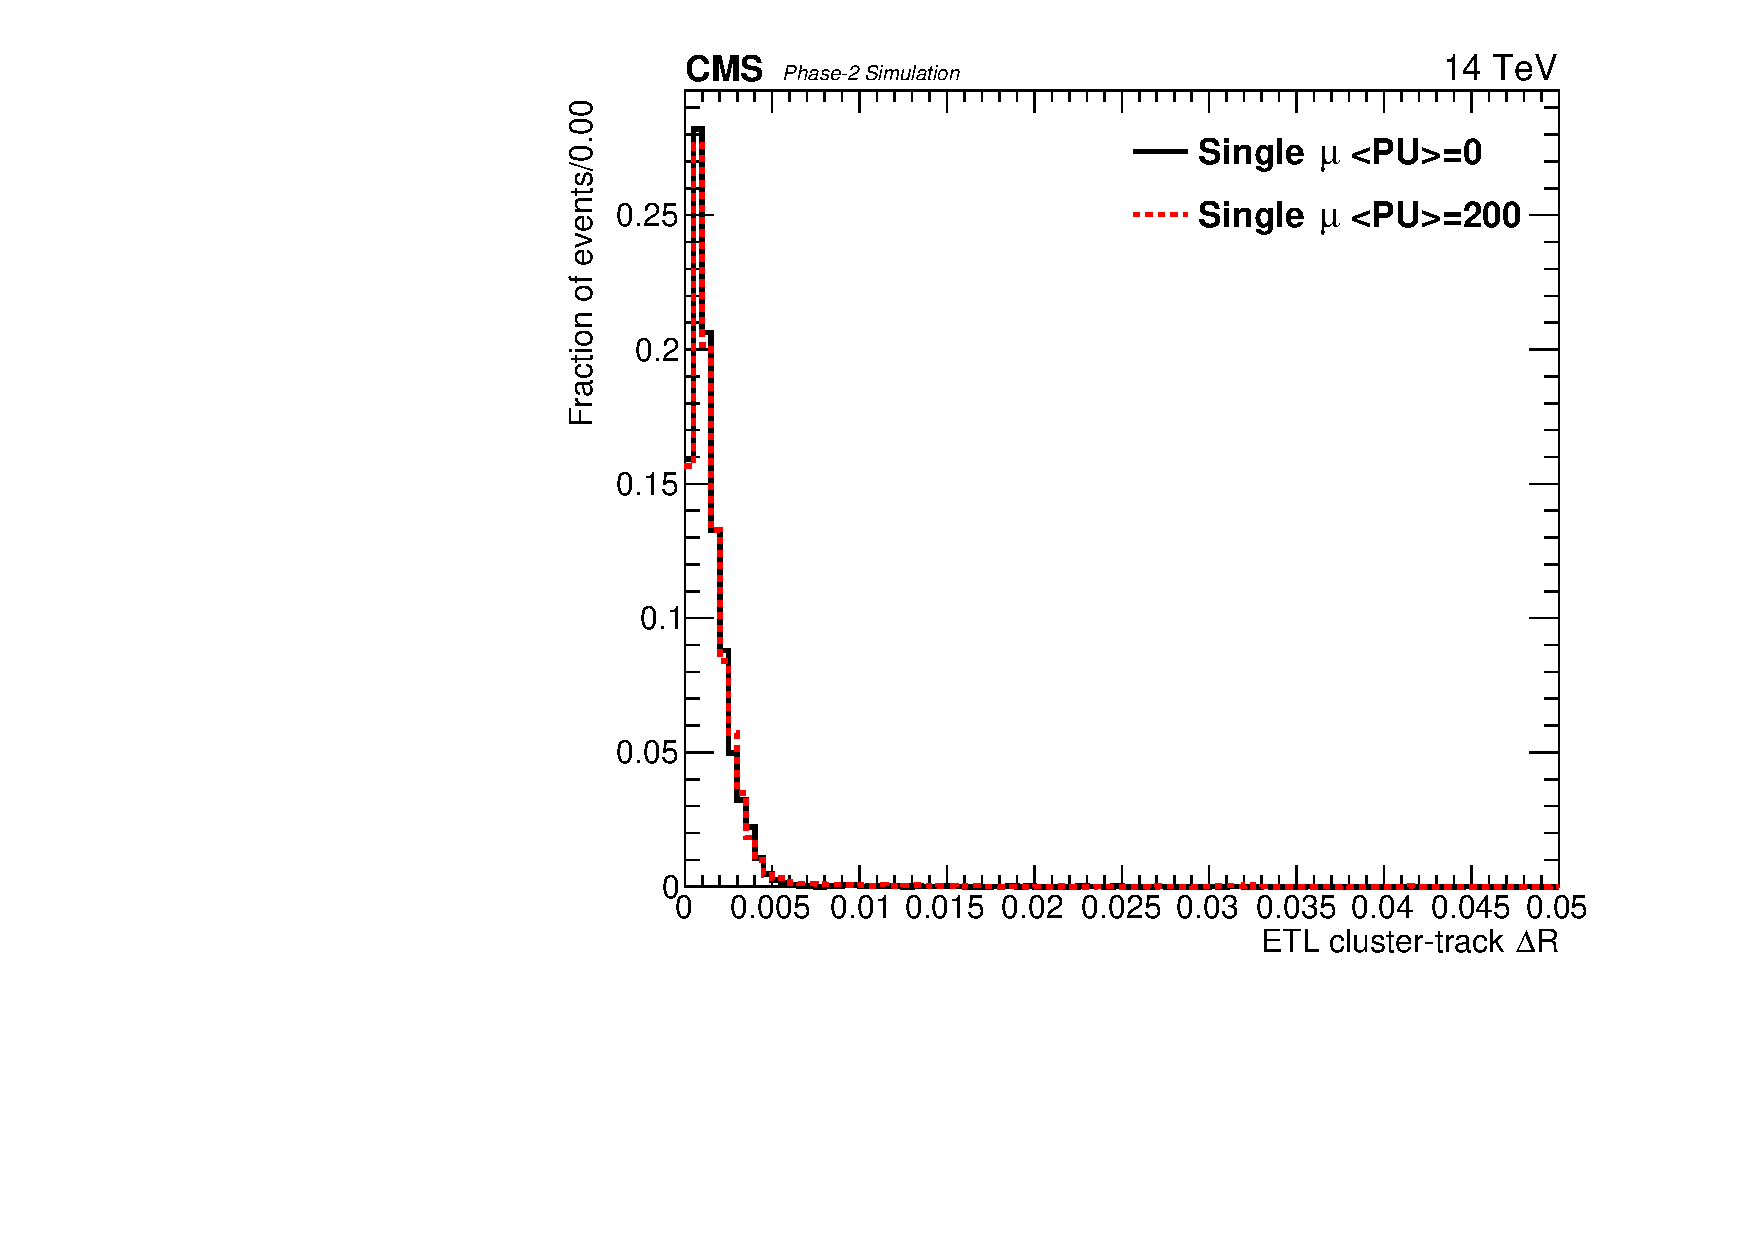
\includegraphics[width=0.48\textwidth]{fig/performance/ClusterAndTracks/noPreliminary/ETLbestCluster_DR_muPUcomp-4.pdf}
%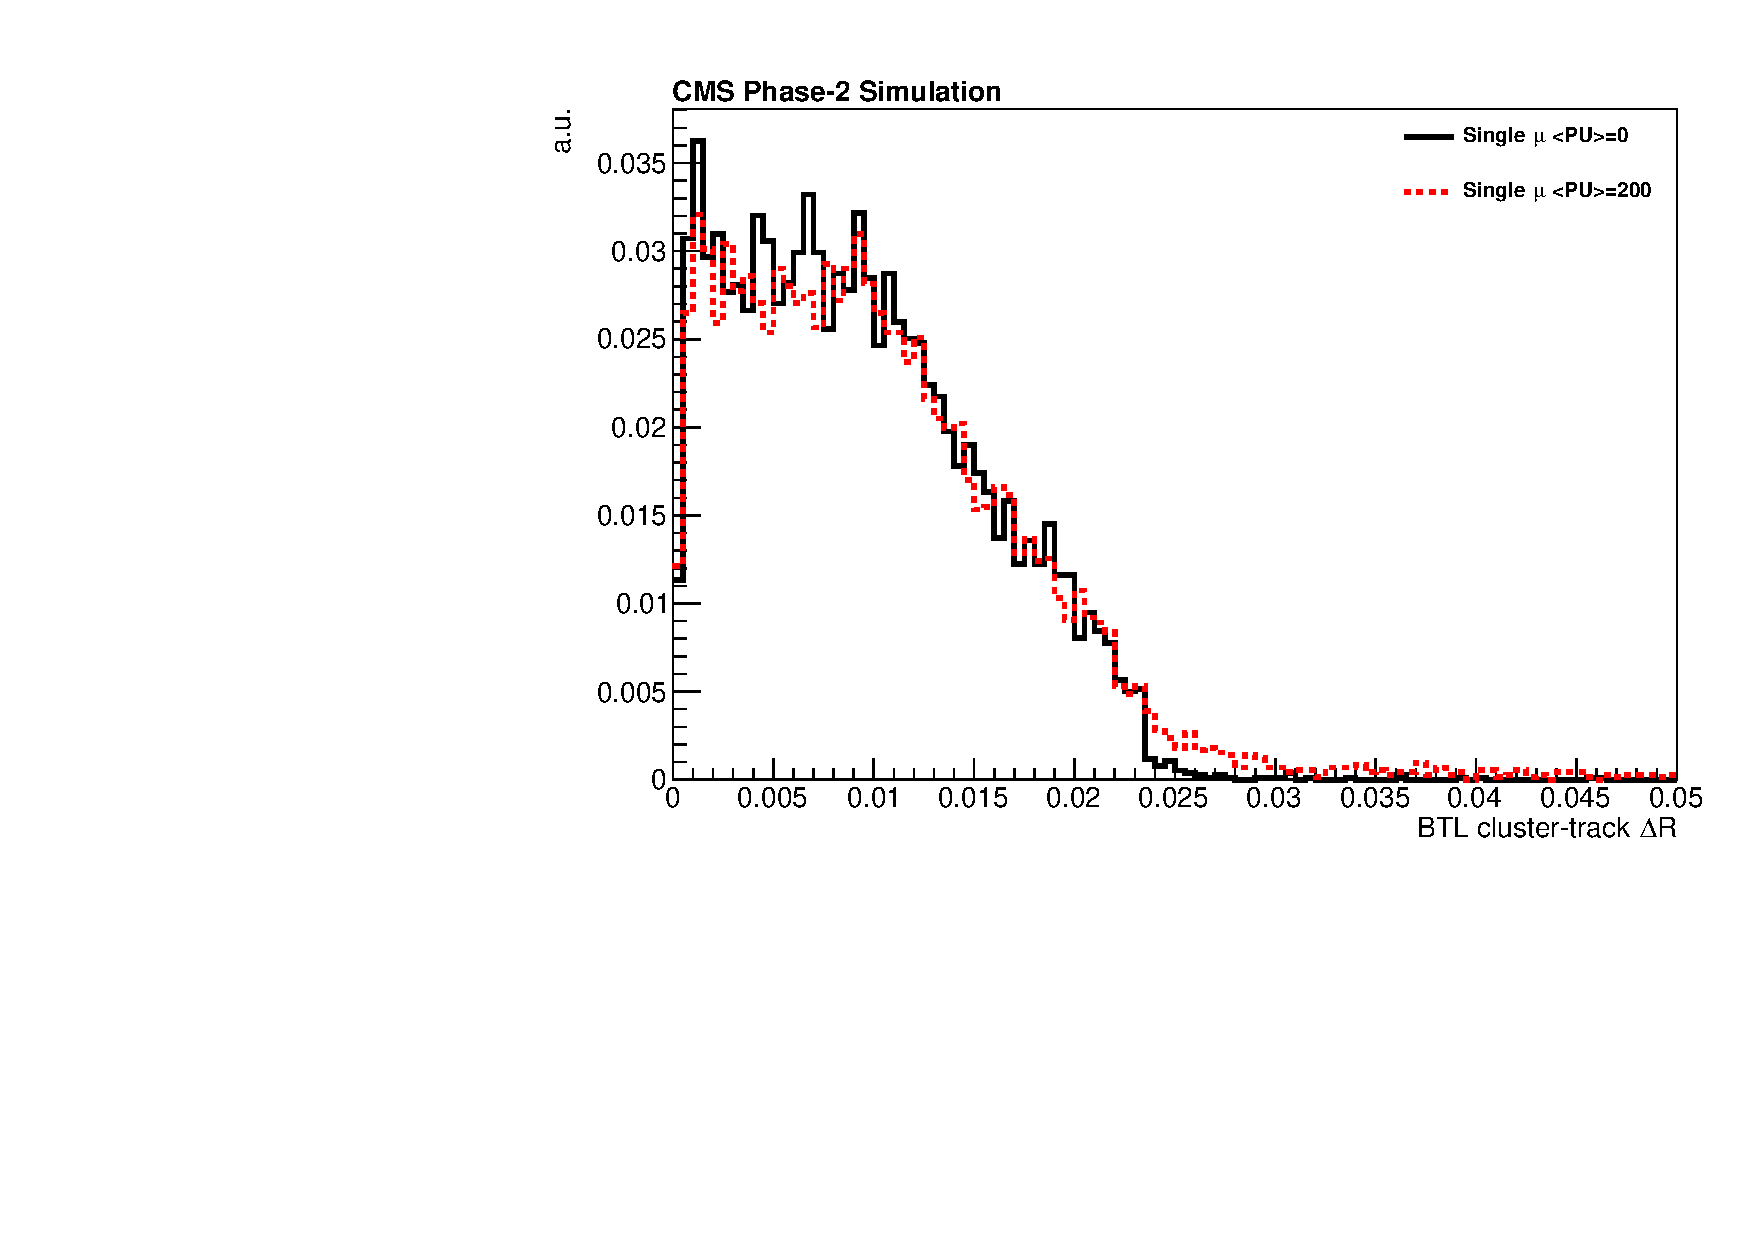
\includegraphics[width=0.32\textwidth]{fig/performance/ClusterAndTracks/BTLbestCluster_DR_muPUcomp.pdf}
\caption{$\Delta R$ for the best matching cluster for BTL (left) and ETL (right). Single muons with flat $p_{T}$ spectrum in 0.7-10~GeV range are used,  with an average of 200 pile-up events(red dotted line) and without pile-up (black line).}
\label{fig:clusterMuPuComp_DeltaR}
\end{figure}


